\section{Change of Variables in Multiple Integrals}\label{sec:transformations}
We have seen in Sections \ref{sec:double_int_polar} and \ref{sec:cylindrical_spherical} that switching to a different coordinate system can be a powerful tool. Integrals that are intractable (or even impossible) in one coordinate system can become straightforward in another. 
\mnote{.8}{\textbf{Note:} Recall Exercise \ref{13_03_ex_15} in Section \ref{sec:double_int_polar}: the function $f(x,y) = e^{-x^2-y^2}$ is impossible to integrate in rectangular coordinates (at least, by finding antidervatives in terms of elementary functions), but switching to polar coordinates results in an integral that can be evaluated using a simple substitution.}

Changing from rectangular coordinates to  polar, or cylindrical, or spherical coordinates, are special cases of a general process known as a \sword{change of variables} \index{change of variables}\index{transformation} or \sword{transformation}. A change of variables should be considered in any situation where we are presented with an integral that is difficult to evaluate in rectangular coordinates.

Our goals in this section are as follows:
\begin{itemize}
\item Understand how a change of variables affects the area element $dA$ in a double integral, or the volume element $dV$ in a triple integral.
\item Derive a general change of variables formula for multiple integrals that works for any suitable change of coordinates, including the ones we have already seen in Sections \ref{sec:double_int_polar} and \ref{sec:cylindrical_spherical}.
\item Develop some basic guiding principles for knowing when a change of variables should be considered, and how to define the corresponding transformation. 
\end{itemize}

One of the situations that should be covered by our general change of variables formula is that of substitution for a definite integral in one variable, as encountered in Section \ref{sec:substitution1}, way back in Calculus I. Of course, for a definite integral in one variable, there is only one type of region of integration: a closed interval $[a,b]$. For single integrals, our only consideration when making a change of variables is the function being integrated. Recall that substitution -- at least, for indefinite integrals -- is essentially an attempt to reverse the Chain Rule: given
\[
\int_a^b f(T(u))T'(u)\,du,
\]
we set $x=T(u)$, compute the differential $dx = T'(u)\,du$, and set
\begin{equation}\label{eqn_single_sub}
\int_a^b f(T(u))T\primeskip'(u)\,du = \int_{T(a)}^{T(b)}f(x)\,dx.
\end{equation}
\mnote{.5}{\textbf{Note:} We have reversed the roles of $x$ and $u$ as they typically appear in Calculus I. This may seem strange in this context, but it's in keeping with the way the change of variables formula in several variables is usually presented.}
The formula we seek will be a generalization of this result, with one notable change in perspective: for multiple integrals, it is often the \emph{region of integration} that creates most of the difficulty, and not the function being integrated. (In one variable, one closed interval is transformed into another, and we apply the Fundamental Theorem of Calculus.) What we will find is that in most cases, we start on the \emph{right} hand side of our analogue of Equation \eqref{eqn_single_sub}, and move to the left. 

\mnote{.25}{For double and triple integrals, it will be important to understand how both the function \emph{and} the region of integration are transformed. For single integrals, the Fundamental Theorem of Calculus (Theorem \ref{thm:FTC2}) lets us gloss over some of the details we'll now need to consider. In particular, we don't really need to pay any attention to the interval over which we're integrate in a single integral, as long as we can come up with an antiderivative.}


Changing from polar coordinates can be viewed as the process of writing our rectangular coordinates $(x,y)$ in terms of new variables $r$ and $\theta$:
\begin{align*}
x(r,\theta) & = r\cos\theta\\
y(r,\theta) & = r\sin\theta,
\end{align*}
or conversely, as defining new variables $r$ and $\theta$ as functions of the old variables $x$ and $y$:
\begin{align*}
r(x,y) & = \sqrt{x^2+y^2}\\
\theta(x,y) & = \arctan(y/x).
\end{align*}

We can think of the polar coordinate transformation as a change of variables, where we define new variables in terms of old ones, but we could also think of it as a \emph{function} from the plane $\mathbb{R}^2$ to itself. That is, we have a mapping
\begin{align*}
T:  D&\subseteq \mathbb{R}^2\to \mathbb{R}^2\\
(x,y) &= T(r,\theta) = (r\cos\theta,r\sin\theta),
\end{align*}
where $D$ is some subset of $\mathbb{R}^2$ (with coordinates labelled by $r$ and $\theta$), and the codomain is $\mathbb{R}^2$ with usual $(x,y)$ coordinates. As we know from Section \ref{sec:double_int_polar}, the polar coordinate transformation $T$ given above transforms a rectangle such as $D=[0,3]\times [0,2\pi]$ into a disk -- in this case, the set of points $(x,y)$ with $x^2+y^2\leq 9$, as shown in Figure \ref{fig:polar_trans1} below.\\

\mnote{.75}{\textbf{Note:} Polar coordinates are a very common choice of coordinate system, because they are well adapted to situations with circular symmetry, a common assumption in many physical problems. They are also natural from a navigational perspective. However, the polar coordinate transformation is a bit unusual, in that it violates some of the principles we will require below for a general transformation: the transformation is not one-to-one, for example, and since we often allow $r<0$ (recall Section \ref{sec:polar_intro}, the inverse transformation (from polar to rectangular) technically isn't even a function! However, we're willing to overlook these defects due to the ubiquity and usefulness of the polar coordinate system.}

\ifthenelse{\isodd{\thepage}}{}{\noindent\hskip-60pt}\noindent\begin{minipage}{\textwidth}
\begin{center}
\begin{tabular}{ccc}
\begin{tikzpicture}
\begin{axis}[width=\marginparwidth+25pt,%
tick label style={font=\scriptsize},axis y line=middle,axis x line=middle,name=myplot,axis on top,%
			xtick={1,2,3,4,5,6,7,8,9},% 
%			extra x ticks={3.14,1.57},
%			extra x tick labels={$\pi$,$\pi/2$},
			ytick={1,2,3,4,5,6,7,8,9},
			%minor y tick num=1,%extra y ticks={-5,-3,...,7},%
%			minor x tick num=4,
			ymin=-0.5,ymax=10,%
			xmin=-0.5,xmax=10%
]

\addplot [name path=top,black,domain=0:3,thick] ({x},{6.28});
\addplot [name path=bottom, black, domain=0:3,thick] ({x},{0});
\addplot [black,domain=0:6.28,thick] ({0},{x});
\addplot [black,domain=0:6.28,thick] ({3},{x});
\addplot [color=gray!20] fill between [of=top and bottom, soft clip={domain=0:3}];
\end{axis}

\node [right] at (myplot.right of origin) {\scriptsize $r$};
\node [above] at (myplot.above origin) {\scriptsize $\theta$};


\end{tikzpicture}
& 
\begin{tikzpicture}
\draw [<-] (2,3.75) arc (45:135:1.1cm);
\node [above] at (1.2,4) {$T$};
\node [below] at (1,2) {};
\end{tikzpicture}
&
\begin{tikzpicture}
\begin{axis}[width=0.9\marginparwidth,height=0.9\marginparwidth,
scale only axis,%
tick label style={font=\scriptsize},axis y line=middle,axis x line=middle,name=myplot,axis on top,%
			xtick={-3,-2,-1,1,2,3},% 
%			extra x ticks={3.14,1.57},
%			extra x tick labels={$\pi$,$\pi/2$},
			ytick={-3,-2,-1,1,2,3},
			%minor y tick num=1,%extra y ticks={-5,-3,...,7},%
%			minor x tick num=4,
			ymin=-3.5,ymax=4,%
			xmin=-3.5,xmax=4%
]

\addplot [name path=top,black,domain={-3:3},samples=100,thick] {sqrt(9-x^2)};
\addplot [name path=bottom, black, domain={-3:3},samples=100,thick] {-sqrt(9-x^2)};
\addplot [color=gray!20] fill between [of=top and bottom, soft clip={domain={-3:3}}];
\end{axis}
\node [right] at (myplot.right of origin) {\scriptsize $x$};
\node [above] at (myplot.above origin) {\scriptsize $y$};
\end{tikzpicture}
\end{tabular}
\end{center}
\captionsetup{type=figure}
\caption{Transforming a rectangle to a disk using polar coordinates.}
\label{fig:polar_trans1}
\end{minipage}\\

\medskip

It is interesting to pause and consider what happens to the four sides of the rectangle $D$ in the transformation above. (As we'll see, this particular transformation exhibits some behaviour we usually prefer to avoid!). First, the
side with $r=0$ is collapsed to a single point: the origin. The side with $r=3$ forms the entire perimeter of the circle. What happens to the sides $\theta=0$ and $\theta=2\pi$? They both get sent to the line segment from $(0,0)$ to $(3,0)$! 

These observations let us imagine transformation as a physical process: first, the left side of the rectangle is shrunk down to a single point, while the right side is simultaneously stretched by a factor of 3. (Vertical lines in between are stretched/shrunk by a factor of $r$, with $0\leq r\leq 3$.) The top of the rectangle is then bent around until it joins with the bottom.

It is perhaps easier to picture the transformation for a domain of the form $[a,b]\times [\alpha,\beta]$, with $0<a< b$ and $0\leq \alpha<\beta< 2\pi$. The case $r\in [1,3]$, $\theta\in [\pi/6, \pi/3]$ is pictured in Figure \ref{fig:polar_trans2} below.\pagebreak

\ifthenelse{\isodd{\thepage}}{}{\noindent\hskip-60pt}\noindent\begin{minipage}{\textwidth}
\begin{center}
\begin{tabular}{ccc}
\begin{tikzpicture}
\begin{axis}[width=\marginparwidth+25pt,%
tick label style={font=\scriptsize},axis y line=middle,axis x line=middle,name=myplot,axis on top,%
			xtick={1,2,3},% 
%			extra x ticks={3.14,1.57},
%			extra x tick labels={$\pi$,$\pi/2$},
			ytick={1,2},
			%minor y tick num=1,%extra y ticks={-5,-3,...,7},%
%			minor x tick num=4,
			ymin=-0.5,ymax=2.5,%
			xmin=-0.5,xmax=3.5%
]

\addplot [name path=top,black,domain=1:2,thick] ({x},{1.047});
\addplot [name path=bottom, black, domain=1:2,thick] ({x},{0.523});
\addplot [black,domain=0.523:1.047,thick] ({1},{x});
\addplot [black,domain=0.523:1.047,thick] ({2},{x});
\addplot [color=gray!20] fill between [of=top and bottom, soft clip={domain=1:2}];
\end{axis}

\node [right] at (myplot.right of origin) {\scriptsize $r$};
\node [above] at (myplot.above origin) {\scriptsize $\theta$};


\end{tikzpicture}
& 
\begin{tikzpicture}
\draw [<-] (2,3.75) arc (45:135:1.1cm);
\node [above] at (1.2,4) {$T$};
\node [below] at (1,2) {};
\end{tikzpicture}
&
\begin{tikzpicture}
\begin{axis}[width=\marginparwidth+25pt,%
tick label style={font=\scriptsize},axis y line=middle,axis x line=middle,name=myplot,axis on top,%
			xtick={1,2,3},% 
%			extra x ticks={3.14,1.57},
%			extra x tick labels={$\pi$,$\pi/2$},
			ytick={1,2,3},
			%minor y tick num=1,%extra y ticks={-5,-3,...,7},%
%			minor x tick num=4,
			ymin=-0.2,ymax=3.5,%
			xmin=-0.2,xmax=3.5%
]
\addplot[data cs=polar, domain=30:60, samples=20, black, thick, name path=out](x,{2});
\addplot[data cs=polar, domain=30:60, samples=20, black, thick, name path=in](x,{1});
\addplot[gray,dashed,domain=0:2.5]{0.57735*x};
\addplot[black,thick,domain=0.866:1.732]{0.57735*x};
\addplot[gray,dashed,domain=0:1.7]{1.732*x};
\addplot[black,thick,domain=0.5:1]{1.732*x};

\addplot[color=gray!20] fill between [of=out and in];
\end{axis}

\node [right] at (myplot.right of origin) {\scriptsize $x$};
\node [above] at (myplot.above origin) {\scriptsize $y$};


\end{tikzpicture}
\end{tabular}
\end{center}
\captionsetup{type=figure}
\caption{Transforming a rectangle to an annular portion using polar coordinates.}
\label{fig:polar_trans2}
\end{minipage}\\

\medskip

Given a region $R$ in the plane and an integral $\displaystyle\iint_R f(x,y)\,dA$, we will look for a domain $D\subseteq \mathbb{R}^2$ and a function $T:D\to \mathbb{R}^2$ of the form
\[
(x,y) = T(u,v) = (h(u,v),k(u,v))
\]
that maps $D$ onto $R$, which can be used to simplify our integral. 

Definition \ref{def:transformation} below specifies the properties we require for a function $T:D\subseteq \mathbb{R}^n\to\mathbb{R}^n$ to be used to define a change of variables. To explain some of those properties, we will need the following definitions.\\

\mnote{.6}{\textbf{Note:} The notation $f:A\to B$ is commonly used in mathematics when we want to indicate that a function $f$ has a particular domain $A$ and codomain $B$. We usually do not see this notation in calculus, since the domain is always a subset of $\mathbb{R}^n$ for some $n$, and understood to be the largest set of values for which the function is defined.

Note however that the choice of domain is part of the definition of a function, and it can significantly affect important properties of that function, such as being one-to-one: recall the definition of the inverse trigonometric functions in Section \ref{sec:deriv_inverse_function}.}

\definition{def:image}{The image of a point or set}{
Let $D\subseteq \mathbb{R}^n$ be any subset, and let $F:D\to \mathbb{R}^m$ be a function. For any point $\mathbf{x}\in D$, the \sword{image}\index{image!of a point} of $\mathbf{x}$ under $F$ is the point $\mathbf{y}=F(\mathbf{x})$ in the range of $F$.

For any subset $C\subseteq D$, the \sword{image}\index{image!of a subset} of $C$ under $F$ is denoted $F(C)$ and defined by
\[
F(C) = \{F(\mathbf{x})\,|\, \mathbf{x}\in C\}.
\]
In other words, $\mathbf{y}\in F(C)$ if and only if $\mathbf{y}$ is the image of $\mathbf{x}$ for some $\mathbf{x}\in C$. 

In particular, we denote the range (or \sword{image}) of $F$ by $F(D)$.}\\

\definition{def:121_onto}{One-to-one and onto functions}{
Let $A\subseteq \mathbb{R}^n$, let $B\subseteq \mathbb{R}^m$, and let $T:A\to B$ be a function. \index{one-to-one}\index{onto}
\begin{itemize}
\item We say that $T$ is \sword{one-to-one} if no two points in $A$ have the same image. That is, for any $\mathbf{x}_1,\mathbf{x}_2\in A$, if $\mathbf{x}_1\neq \mathbf{x}_2$, then $T(\mathbf{x}_1)\neq T(\mathbf{x}_2)$.
\item We say that $T$ is \sword{onto} if the range of $T$ is $B$; that is, if $T(A)=B$.
\end{itemize}
}

\mnote{.4}{\textbf{Note:} To avoid clutter throughout this section, we will use boldface variables as shorthand for points in $\mathbb{R}^n$. For example, we will write $\mathbf{x}$ instead of $(x_1,x_2,\ldots, x_n)$}


%(Of course, this is not quite as simple as just setting $x=h(u,v)$ and $y=k(u,v)$. We know from Section \ref{sec:double_int_polar} that the area element $dA$ is also transformed by a change of variables.)

\enlargethispage{2\baselineskip}

A function used for a change of variables is called a \emph{transformation}. Such functions need to be one-to-one, except possibly on the boundary of their domain, and they need to be continuously differentiable. (See Definition \ref{def:transformation} below.) One of the important properties of a transformation, which we will justify later in this section (see Theorem \ref{thm:boundary_transform}, is that the boundary of a closed, bounded domain is mapped to the boundary of the range. This observation is key to visualizing the effect of a transformation, as the following example illustrates.\\

\example{ex_trans_boundary}{Describing the effect of a transformation}{
Let $D\subseteq \mathbb{R}^2$ be the rectangle defined by $1\leq u\leq 2$ and $0\leq v\leq 1$. Determine the range of the function $T:D\to\mathbb{R}^2$ defined by
\[
(x,y)=T(u,v)=(uv, u^2+2v^2).
\]}
{The function $T$ is continuously differentiable, since $x=4uv$ and $y=u^2+v^2$ both have continuous first-order partial derivatives with respect to $u$ and $v$. Showing that $T$ is one-to-one is a mess of algebra that we omit here. From these properties, we can conclude that the boundary of $D$ will be transformed to the boundary of $T(D)$.

\mnote{.65}{\textbf{Note:} While it is important to know that our function is one-to-one, we will usually not ask you to check this fact. However, you should make sure you're aware of what can go wrong if this property is not satisfied: see the discussion following Definition \ref{def:transformation}.}

Now, let's see what happens to the boundary of $D$. The boundary consists of four line segments:
\begin{enumerate}
\item The segment $u=1$, $0\leq v\leq 1$.
\item The segment $u=2$, $0\leq v\leq 1$.
\item The segment $1\leq u\leq 2$, $v=0$.
\item The segment $1\leq u\leq 2$, $v=1$.
\end{enumerate}
On the first segment, $x=v$ and $y=1+v^2$, with $0\leq v\leq 1$. Eliminating the parameter $v$ gives us portion of the parabola $y=1+x^2$ from $(0,1)$ to $(1,2)$.

For the second segment we have $x=2v$ and $y=4+v^2$. This is the part of the parabola $y=4+\frac14 x^2$ from $(0,4)$ to $(2,5)$.

The third segment has $x=0$ and $y=u^2$, for $1\leq u\leq 2$. This is the portion of the $y$ axis from $(0,1)$ to $(0,4)$.

Finally, the fourth segment is given by $x=u$, $y=u^2+1$, for $1\leq u\leq 2$. This is again the parabola $y=1+x^2$, but this time $1\leq x\leq 2$.

The resulting region is plotted in Figure \ref{fig:trans_map1}. Interestingly, two of the four sides of the rectangle bounding $D$ were mapped to (different portions of) the same curve.
}\\

\mtable{.4}{Plotting the image of the function $T$ in Example \ref{ex_trans_boundary}}{fig:trans_map1}{
\ifthenelse{\boolean{colour}}{
\begin{tikzpicture}
\begin{axis}[width=\marginparwidth+25pt,%
tick label style={font=\scriptsize},axis y line=middle,axis x line=middle,name=myplot,%
			xtick={1,2,3},% 
%			extra x ticks={3.14,1.57},
%			extra x tick labels={$\pi$,$\pi/2$},
			ytick={1,2,3,4,5},
			%minor y tick num=1,%extra y ticks={-5,-3,...,7},%
%			minor x tick num=4,
			ymin=-0.5,ymax=5.2,%
			xmin=-0.5,xmax=3.2%
]

\addplot [name path=a,ultra thick,color=blue,domain=0:1] {x^2+1};

\addplot [name path=b,ultra thick,color=red,domain=1:2] {x^2+1};

\addplot [name path=c,ultra thick, color=blue,domain=0:2] {0.25*x^2+4};

\addplot [color=red,ultra thick,domain=1:4]({0},{x});

\addplot [color=blue!20] fill between [of=a and c, soft clip={domain=0:1}];
\addplot [color=blue!20] fill between [of=b and c, soft clip={domain=1:2}];
\end{axis}

\node [right,color=blue] at (1,3.7) {$u=2$};
\node [right,color=red] at (3,2.5) {$v=1$};
\node [right,color=blue] at (1,0.9) {$u=1$};
\node [left,color=red] at (0.2,2) {$v=0$};

\node [right] at (myplot.right of origin) {\scriptsize $x$};
\node [above] at (myplot.above origin) {\scriptsize $y$};


\end{tikzpicture}}
{
\begin{tikzpicture}
\begin{axis}[width=\marginparwidth+25pt,%
tick label style={font=\scriptsize},axis y line=middle,axis x line=middle,name=myplot,%
			xtick={1,2,3},% 
%			extra x ticks={3.14,1.57},
%			extra x tick labels={$\pi$,$\pi/2$},
			ytick={1,2,3,4,5},
			%minor y tick num=1,%extra y ticks={-5,-3,...,7},%
%			minor x tick num=4,
			ymin=-0.5,ymax=5.2,%
			xmin=-0.5,xmax=3.2%
]

\addplot [name path=a,ultra thick,color=gray,domain=0:1] {x^2+1};

\addplot [name path=b,ultra thick,color=black,domain=1:2] {x^2+1};

\addplot [name path=c,ultra thick, color=gray,domain=0:2] {0.25*x^2+4};

\addplot [color=black,ultra thick,domain=1:4]({0},{x});

\addplot [color=gray!20] fill between [of=a and c, soft clip={domain=0:1}];
\addplot [color=gray!20] fill between [of=b and c, soft clip={domain=1:2}];
\end{axis}

\node [right,color=gray] at (1,3.7) {$u=2$};
\node [right,color=black] at (3,2.5) {$v=1$};
\node [right,color=gray] at (1,0.9) {$u=1$};
\node [left,color=black] at (0.2,2) {$v=0$};

\node [right] at (myplot.right of origin) {\scriptsize $x$};
\node [above] at (myplot.above origin) {\scriptsize $y$};


\end{tikzpicture}
}}

This example is interesting, in that two of the four sides of our rectangular domain were mapped to the same curve. Note also that -- without explicitly solving for the inverse function, giving $u$ and $v$ as functions of $x$ and $y$ -- we can see that lines of constant $x$ in the $u,v$ plane are circles, and lines of constant $y$ are hyperbolas.

One other observation is worthy of note: we mentioned above that we will be primarily concerned with finding transformations that can be used to simplify a double integral. Suppose we were given a double integral over $R=T(D)$, as pictured in Figure \ref{fig:trans_map1}. We probably wouldn't even consider a change of variables in this case, unless one was needed for the function being integrated: the region can be described by the inequalities
\[
1+x^2\leq y\leq 4+\frac14 x^2, \text { where } 0\leq x\leq 2.
\]
We already learned how to deal with such regions at the beginning of this Chapter, and in any case, it's unlikely that anyone looking at this region would come up with the transformation we just considered.

We're ready to move on, and describe the effect of a change of variables on an integral.
We begin with an observation from single variable calculus. Consider the definition of a definite integral as a limit of Riemann sums. When we make a change of variables $x=T(u)$ in a single integral, a partition of $[a,b]$ given by $a=u_0<u_1<\cdots <u_n=b$ is transformed into a partition $x_0=T(u_0),x_1=T(u_1), \ldots, x_n=T(u_n)$. (As long as $T'(u)>0$, we have $x_0<x_1<\cdots x_n$.) The transformation affects the size of the subintervals in the partition: from Section \ref{sec:differentials}, we know that $\Delta x_i \approx T\primeskip' (u_i)\Delta x_i$. Thus, the derivative tells us how the size of each subinterval changes under the transformation.

This gives us a way of thinking about the geometric effect of a substitution. In the integral $\displaystyle\int_{T(a)}^{T(b)}f(x)\,dx$, the subintervals in a partition (thought of as the width of the rectangles in a Riemann sum)  are stretched/shrunk horizontally by a factor given by the derivative $T'(u)$ of the transformation function $g(u)$. In the integral $\displaystyle\int_a^b f(T(u))T'(u)\,du$, the derivative $T'(u)$ is part of the integrand, and therefore our horizontal stretch/shrink becomes a vertical stretch/shrink. Of course, the area of a rectangle changes by the same amount regardless of whether the stretch/shrink is horizontal or vertical.

\mnote{.4}{\textbf{Note:} In the discussion given here, we will stick to two variables for simplicity of presentation. However, everything we do for double integrals works equally well for triple integrals in three variables.}

\mnote{.25}{\textbf{Note:} Another common notation for the Jacobian is 
\[
J_T(u,v) = \frac{\partial (x,y)}{\partial (u,v)}.
\]
This notation is intended to be reminiscent of the Leibniz form of the chain rule when $T$ is used to define a change of variables: we have the mnemonic devices
\begin{align*}
dx %= \frac{dx}{du}du\\ dx\,dy &= \frac{\partial(x,y)}{\partial (u,v)}\,du\,dv\\ dx\,dy\,dz &= \frac{\partial (x,y,z)}{\partial (u,v,w)}\,du\,dv\,dw
\end{align*}
for a change of variables in single, double, and triple integrals, respectively.}

Similarly, when we do a change of variables in two or three variables, we need a measure of how the size of each subregion in a partition changes under change of variables. This measure is given by an object known as the \emph{Jacobian}.\\

\definition{def:jacobian}{The Jacobian of a transformation}{
Let $D\subseteq \mathbb{R}^2$ be a subset of the plane, described with coordinates $(u,v)$. Let $T:D\subseteq \mathbb{R}^2\to \mathbb{R}^2$ be given by
\[
T(u,v)=(f(u,v),g(u,v)),
\]
where $f$ and $g$ are continuously differentiable on $D$. The \sword{Jacobian}\index{Jacobian} is the function $J_T:D\to \mathbb{R}$ defined by
\[
J_T(u,v)=\det\begin{bmatrix}f_u(u,v)&f_v(u,v)\\g_u(u,v)&g_v(u,v)\end{bmatrix}.
\]
If we define $x=f(u,v)$ and $y=g(u,v)$, we can write the Jacobian as 
\[
J_T(u,v) = \det\begin{bmatrix}x_u&x_v\\y_u&y_v\end{bmatrix} = \det\begin{bmatrix}\frac{\partial x}{\partial u}&\frac{\partial x}{\partial v}\\[5pt] \frac{\partial y}{\partial u}&\frac{\partial y}{\partial v}\end{bmatrix}.
\]
}\\

In the case of a transformation $T:D\subseteq \mathbb{R}^3\to\mathbb{R}^3$, with $(x,y,z)=T(u,v,w)$, the definition of the Jacobian is similar, except that we need to compute the determinant of a $3\times 3$ matrix. If you read Section \ref{sec:deriv_matrix} on the definition of the derivative as a matrix of partial derivatives, you probably recognize the matrix whose determinant gives us the Jacobian: it's the derivative matrix! One therefore could write
\[
J_T(u,v) = \det DT(u,v)
\]
for the Jacobian, and this formula is valid in any dimension. In fact, we can even use this definition for single integrals: a $1\times 1$ matrix is just a number, and the determinant does nothing to that number, and of course, the derivative of a function of one variable is the same as always.\pagebreak



\example{ex_jacobian1}{Computing the Jacobian of a transformation}{
Compute the Jacobian of the transformation $(x,y)=T(u,v)$ given by
\[
x = 7u-3v \quad y = -4u+2v.
\]}
{We apply Definition \ref{def:jacobian} directly:
\[
J_T(u,v) = \det\begin{bmatrix}x_u(u,v)&x_v(u,v)\\y_u(u,v)&y_v(u,v)\end{bmatrix} = \det\begin{bmatrix}7&-3\\-4&2\end{bmatrix} = 7(2)-(-3)(-4)=2.
\]
\vskip-\baselineskip}\\

In this case, the Jacobian is a constant function. This is the case whenever $x$ and $y$ are linear functions of $u$ and $v$., but not true in general. We'll look at the case of linear transformations in more detail after a few more examples.\\

\example{ex_jacobian2}{Computing the Jacobian of a transformation}{
Compute the Jacobian of the transformation given by
\[
T(u,v) = (\sqrt[3]{x^2y}, \sqrt[3]{xy^2}).
\]}
{Again, this is a direct application of the definition, but we should be clever about how we compute our partial derivatives. Our transformation defines $x=\sqrt[3]{x^2y}$ and $y=\sqrt[3]{xy^2}$. If we blindly push forward with the partial derivatives as written, we get a mess. For example, if we get a little too excited, we might do something like:
\[
x_u(u,v) = \frac{\partial}{\partial u}(\sqrt[3]{x^2y}) = \frac{1}{3}(x^2y)^{-2/3}(2xy),
\]
with similar results for the other four partial derivatives. Instead, let's first simplify using laws of exponents:
\begin{align*}
x(u,v) &= \sqrt[3]{x^2y} = (x^2y)^{1/3} = x^{2/3}y^{1/3} \quad\text{ and}\\
y(u,v) &= \sqrt[3]{xy^2} = (xy^2)^{1/3} = x^{1/3}y^{2/3}.
\end{align*}
Now we only need the power rule to compute our partial derivatives, and we find
\begin{align*}
J_T(u,v) &= \det\begin{bmatrix}x_u(u,v)&x_v(u,v)\\y_u(u,v)&y_v(u,v)\end{bmatrix} \\
&= \det\begin{bmatrix}\frac23 x^{-1/3}y^{1/3}& \frac13 x^{2/3}y^{-2/3}\\ \frac13 x^{-2/3}y^{2/3}& \frac23 x^{1/3}y^{-1/3}\end{bmatrix}\\
&= \left(\frac23 x^{-1/3}y^{1/3}\right)\left( \frac23 x^{1/3}y^{-1/3}\right)-\left(\frac13 x^{2/3}y^{-2/3}\right)\left(\frac13 x^{-2/3}y^{2/3}\right)\\
&=\frac49 -\frac19 = \frac13.
\end{align*}
\vskip-1.5\baselineskip}\\

Interestingly enough, the Jacobian turns out to be constant again, even though the transformation was far from being linear. Let's try one more.\\

\example{ex_jacobian3}{Computing the Jacobian of a transformation}{
Compute the Jacobian of the transformation 
\[
x= 4u^2-v^2 \quad y = 2u^2+3v^2.
\]}
{Computing the Jacobian in this case is straightforward:
\[
J_T(u,v) = \det\begin{bmatrix}x_u(u,v)&x_v(u,v)\\y_u(u,v)&y_v(u,v)\end{bmatrix} = \det\begin{bmatrix} 8u&-2v\\4u&6v\end{bmatrix} 48uv+8uv=56uv.
\]
\vskip-1.5\baselineskip}\\

As hinted at earlier, the Jacobian is important because it appears in the change of variables formula to come. Its role is analogous to that of the derivative $g'(u)$ in Equation \eqref{eqn_single_sub}. We also need the Jacobian to precisely define the type of function that can be used for a change of variables.\\

\definition{def:transformation}{Properties of a transformation}{
Let $D$ and $E$ subsets of $\mathbb{R}^2$, with $D\subseteq \mathbb{R}^2$ described in terms of coordinates $u,v$, and $E\subseteq \mathbb{R}^2$ described in terms of coordinates $x,y$. We say that a function $T:D\to E$ is a \sword{transformation}\index{transformation} if:
\begin{enumerate}
\item $T$ is continuously differentiable.
\item $T$ is one-to-one, and the range of $T$ is $E$.
\item The Jacobian of $T$ does not vanish: $J_T(u,v)\neq 0$ for all $(u.v)\in D$.
\end{enumerate}}\\

\mnote{.4}{\textbf{Note:}  For all three coordinate systems we've studied, the transformation conditions can fail on the boundary of our domain, which we're willing to accept. What would \emph{not} be acceptable is a situation where the transformation conditions fail on a region interior to the domain.

For example, the function $T(r,\theta) = (r\cos\theta,r\sin\theta)$ would not produce an acceptable transformation for domains such as $r\in [-1,1],\, \theta\in [0,2\pi]$ or $r\in [0,2],\, \theta\in [0,3\pi]$. The first traces out the unit disk twice: once for $r<0$, and once for $r>0$. The range of the second transformation is the disk $x^2+y^2\leq 4$, but the upper half of this disk is produced twice: once for $\theta\in [0,\pi]$, and again for $\theta\in [2\pi,3\pi]$.

If we were using these transformations to help compute a double integral over a circular region, we'd get the wrong answer! }

When $D$ is a closed, bounded subset, we can relax Definition \ref{def:transformation} slightly: each of the three conditions above must hold on the interior of $D$, but are allowed to fail on all or part of the boundary. In particular, this is the case for cylindrical, and spherical coordinates:
\begin{itemize}
\item The polar coordinate transformation $x=r\cos\theta, y=r\sin\theta$ is only one-to-one if $r>0$ and $\theta$ belongs to an interval whose length is less than $2\pi$. Note that $J_T(r,\theta)$ vanishes at $r=0$.

Of course, we often use a domain such as $r\in [0,R]$, $\theta = [0,2\pi]$ to describe a disk centred at the origin. The conditions of Definition \ref{def:transformation} fail at $r=0$, and because points with $\theta=0$ get mapped to the same place as points with $\theta = 2\pi$. But these coordinates describe 3 of the 4 sides of the boundary rectangle for our domain, and we allow such boundary defects.

\item The cylindrical coordinate transformation has exactly the same issues as polar coordinates.

\item For spherical coordinates, we take $\rho\geq 0$ and again accept the fact that our transformation is not one-to-one (and the Jacobian is zero) when $\rho=0$. Similarly, we generally allow $\theta\in [0,2\pi]$ and $\varphi\in [0,\pi]$ even though endpoints of these intervals might get sent to the same point.
\end{itemize}


Before we move on to the change of variables formula, we consider one more example that will help clarify the geometry involved in a change of variables.

\pagebreak
\noindent\textbf{\large The Jacobian of a Linear Map}\\

Before we continue to the change of variables formula, let us pause to consider an example that may be familiar to you from a first course in linear algebra.

We saw in Example \ref{ex_jacobian1} that when $x$ and $y$ are linear functions of $u$ and $v$, the Jacobian of the transformation is a constant. What does that constant tell us about the transformation? Here is an example taken from the book Matrix Algebra, by Greg Hartman (one of the APEX authors!), which is sometimes used as part of a textbook for our Math 1410 linear algebra course.

\example{ex_mv_3}{Visualizing a linear function from $\mathbb{R}^2$ to $\mathbb{R}^2$}{Consider the function $T:\mathbb{R}^2\to \mathbb{R}^2$ given by
\[
T(u,v) = (u+4v,2u+3v).
\]
Note that $T$ is linear in both variables. In fact, if we set $(x,y)=T(u,v)$ and represent points by vectors, replacing $(x,y)$ by $\vec{x}=\begin{bmatrix}x\\y\end{bmatrix}$ and $(u,v)$ by $\vec{u}=\begin{bmatrix}u\\v\end{bmatrix}$, then we can write this function as the matrix transformation $\vec{x}=A\vec{u}$, where $A$ is the $2\times 2$ matrix $\begin{bmatrix}1&4\\2&3\end{bmatrix}$. That is:
\[
\begin{bmatrix}x\\y\end{bmatrix} = \begin{bmatrix}1&4\\2&3\end{bmatrix}\begin{bmatrix}u\\v\end{bmatrix}.
\]
To visualize the effect of $T$, plot the vectors representing the four corners of the unit square, before and after they have been multiplied by $A$, where 
\[
A = \begin{bmatrix} 1&4\\2&3\end{bmatrix}.
\] }
{The four corners of the unit square can be represented by the vectors 
\[
\begin{bmatrix}0\\0\end{bmatrix}, \quad \begin{bmatrix}1\\0\end{bmatrix},\quad \begin{bmatrix}1\\1\end{bmatrix},\quad \begin{bmatrix}0\\1\end{bmatrix}.
\]
Multiplying each by $A$ gives the vectors 
\[
\begin{bmatrix}0\\0\end{bmatrix},\quad \begin{bmatrix} 1\\2\end{bmatrix},\quad \begin{bmatrix} 5\\5\end{bmatrix},\quad \begin{bmatrix} 4\\3\end{bmatrix},
\]
respectively. 

%\drawexampleline{ex_mv_3}

The unit square and its transformation are graphed in Figure \ref{fig:mv_3}, where the shaped vertices correspond to each other across the two graphs. Note how the square got turned into some sort of quadrilateral (it's actually a parallelogram). A really interesting thing is how the triangular and square vertices seem to have changed places -- it is as though the square, in addition to being stretched out of shape, was flipped. 
%
%
%

\begin{minipage}{\textwidth}
\begin{center}
\begin{tabular}{cc}
\begin{tikzpicture}
\draw[thick,<->] (-1.2,0) -- (5.2,0) node[right] {$x$};
\draw[thick,<->] (0,-1.2) -- (0,5.2) node[above] {$y$};
\foreach \x in {-1,0,1,2,3,4,5}
	\draw (\x, 2pt) -- (\x, -2pt);
\foreach \x in {-1,1,2,3,4,5}	
	\node at (\x,0) [below] {$\x$};
\foreach \y in {-1,0,1,2,3,4,5}
	\draw (2pt,\y) -- (-2pt,\y);
\foreach \y in {-1,1,2,3,4,5}	
	\node at (0,\y) [left] {$\y$};


\draw (0,0) node (A) {} -- (1,0) node (B) {} -- (1,1) node (C) {} -- (0,1) node (D) {} -- cycle;
\draw [->, ultra thin] (0,.25)--(1,.25);
\draw [->, ultra thin] (0,.5)--(1,.5);
\draw [->, ultra thin] (0,.75)--(1,.75);
\filldraw [black]  (A) circle (2pt);
\filldraw [fill=white,thick]  (B) ++(-2pt,-2pt) rectangle ++(4pt,4pt);
\filldraw [fill=white,thick]  (C) circle (2pt);
\filldraw [fill=white,thick]  (D) ++(-2.5pt,-2.5pt) -- ++(5pt,0pt) -- ++(-2.5pt,5pt) -- cycle;

\end{tikzpicture}&
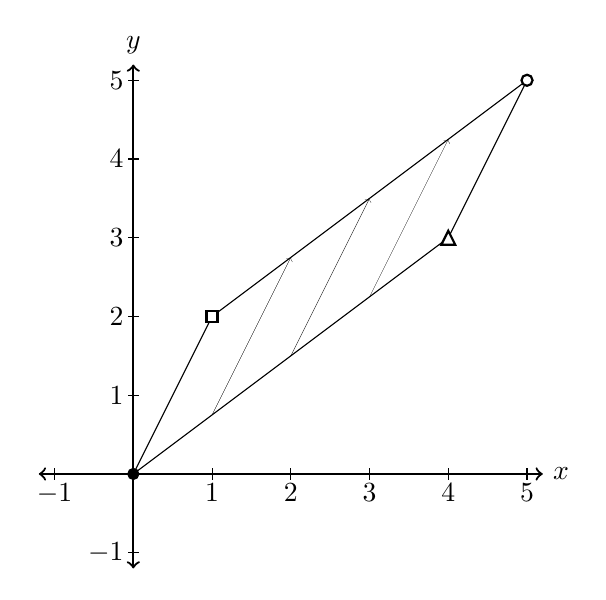
\begin{tikzpicture}
\draw[thick,<->] (-1.2,0) -- (5.2,0) node[right] {$x$};
\draw[thick,<->] (0,-1.2) -- (0,5.2) node[above] {$y$};
\foreach \x in {-1,0,1,2,3,4,5}
	\draw (\x, 2pt) -- (\x, -2pt);
\foreach \x in {-1,1,2,3,4,5}	
	\node at (\x,0) [below] {$\x$};
\foreach \y in {-1,0,1,2,3,4,5}
	\draw (2pt,\y) -- (-2pt,\y);
\foreach \y in {-1,1,2,3,4,5}	
	\node at (0,\y) [left] {$\y$};

\draw (0,0) node (E) {} -- (1,2) node (F) {} -- (5,5) node (G) {} -- (4,3) node (H) {} -- cycle;
\draw [->, ultra thin] (1,.75)--(2,2.75);
\draw [->, ultra thin] (2,1.5)--(3,3.5);
\draw [->, ultra thin] (3,2.25)--(4,4.25);
\filldraw [black]  (E) circle (2pt);
\filldraw [fill=white,thick]  (F) ++(-2pt,-2pt) rectangle ++(4pt,4pt);
\filldraw [fill=white,thick]  (G) circle (2pt);
\filldraw [fill=white,thick]  (H) ++(-2.5pt,-2.5pt) -- ++(5pt,0pt) -- ++(-2.5pt,5pt) -- cycle;

\end{tikzpicture}
\end{tabular}
\end{center}
\captionsetup{type=figure}
\caption{Transforming the unit square by matrix multiplication in Example \ref{ex_mv_3}.}
\label{fig:mv_3}
\end{minipage}\\

How does all this relate to Jacobians and change of variables? First note that the derivative of any linear function is (perhaps not so surprisingly) the matrix that defines it: for $T(u,v) = (u+4v,2u+3v)$, we have
\[
DT(u,v) = \begin{bmatrix}1&4\\2&3\end{bmatrix} = A.
\]
The Jacobian of $T$ is then the determinant of this matrix:
\[
J_T(u,v) = \det A = 1(3)-4(2)=-5.
\]
Let us make a note of a few key points about this example. First, note that in this case, the derivative matrix, (and as a result, the Jacobian) is constant. (This of course is generally true of the derivative for linear functions.)

What happens when we apply the map $T$ to the unit square? The value $J_T(u,v)=-5$ tells us two things:
\begin{itemize}
\item First, the area of the unit square is increased by a factor of 5.
\item Second, the transformation $T$ reverses the \sword{orientation}\index{orientation} of the unit square. This is indicated by the negative value of the determinant. The reversal of orientation is responsible for the ``flipping'' of the square noticed above.
\end{itemize} 
The result of performing the transformation $T$ on the unit square is therefore the following: first, the square is flipped over. Then, the square is stretched out into a parallelogram whose area is 5 times that of the original square.
\mnote{.4}{\textbf{Note:} Recall from linear algebra, that if two vectors $\vec{a}, \vec{b}$ span a parallelogram in the plane, then the determinant of the $2\times 2$ matrix containing $\vec{a}$ and $\vec{b}$ gives the area (up to sign) of the parallelogram.}
}\\

Let us make a couple of remarks about the preceding example. First, note the need for an absolute value around the determinant, to ensure the area computed is positive. This absolute value will be needed in our change of variables formula as well.
\mnote{.2}{\textbf{Note:} Recall the following property for definite integrals in one variable: $\displaystyle \int_a^bf(x)\,dx = -\int_b^af(x)\,dx$. The definite integral is sensitive to the \emph{orientation} of the interval over which the integration is performed. (Left to right or right to left.) Double and triple integrals do not have this sensitivity. We'll see in Section \ref{sec:parametric_surfaces} how information about orientation is reintroduced in the context of vector calculus.}

Second, since our transformation was linear, with constant derivative, the effect on area is the same for any portion of the plane: applying the transformation $T$ to a closed bounded region $D\subseteq \mathbb{R}^2$ of area $A$ will produce a region of area $5A$. For non-linear transformations, the value of the Jacobian (and hence, the effect on area) will vary from point to point.

Before we move on, let's do two more examples, with transformations we've already encountered. In these examples, we'll find that the value of the Jacobian is not a constant.\\

\example{ex_jacobian4}{The Jacobians for polar and spherical coordinate transformations}{
Compute the Jacobian for
\begin{enumerate}
\item The polar coordinate transformation
\[
x = r\cos\theta \quad y = r\sin\theta
\]
\item The spherical coordinate transformation
\[
x = r\cos\theta\sin\varphi \quad y = r\sin\theta\sin\varphi \quad z = r\cos\varphi.
\]
\end{enumerate}}
{
\begin{enumerate}
\item Here we've defined $x$ and $y$ in terms of the coordinates $r$ and $\theta$ instead of $u$ and $v$, but the process is the same:
\begin{align*}
J_T(r,\theta) &= \det\begin{bmatrix}x_r(r,\theta) & x_\theta(r,\theta)\\
y_r(r,\theta) & y_\theta(r,\theta)\end{bmatrix} = \det\begin{bmatrix}
\cos\theta & -r\sin\theta\\ \sin\theta & r\cos\theta\end{bmatrix}\\
& = r\cos^2\theta+r\sin^2\theta = r.
\end{align*}
Interesting. Note that the value of the Jacobian is $r$, which is precisely the correction factor needed in the area element for a double integral when we change from rectangular to polar coordinates. Let's try the spherical coordinate transformation to see if this was merely a coincidence.

\item Although we haven't defined the Jacobian for a change of coordinates in three variables, the process is exactly the same. We form the derivative of the transformation, given by the matrix of partial derivatives, and compute its determinant. We find:
\begin{align*}
J_T(r,\theta,\varphi) &= \det\begin{bmatrix} 
x_\rho(\rho,\theta,\varphi) & x_\theta(\rho,\theta,\varphi) & x_\varphi(\rho,\theta,\varphi)\\
y_\rho(\rho,\theta,\varphi) & y_\theta(\rho,\theta,\varphi) & y_\varphi(\rho,\theta,\varphi)\\
z_\rho(\rho,\theta,\varphi) & z_\theta(\rho,\theta,\varphi) & z_\varphi(\rho,\theta,\varphi)\end{bmatrix}\\
& = \det\begin{bmatrix}
\cos\theta\sin\varphi & -\rho\sin\theta\sin\varphi & \rho\cos\theta\cos\varphi\\
\sin\theta\sin\varphi & \rho\cos\theta\sin\varphi & \rho\sin\theta\cos\varphi\\
\cos\varphi & 0 & -\rho\sin\varphi\end{bmatrix}\\
& = \rho\sin\theta\sin\varphi\begin{vmatrix}
\sin\theta\sin\varphi & \rho\sin\theta\cos\varphi\\
\cos\varphi & -\rho\sin\varphi
\end{vmatrix}\\
&\quad\quad + \rho\cos\theta\sin\varphi\begin{vmatrix}
\cos\theta\sin\varphi & \rho\cos\theta\cos\varphi\\
\cos\varphi &-\rho\sin\varphi
\end{vmatrix}\\
&=\rho\sin\theta\sin\varphi(-\rho\sin\theta(\sin^2\varphi+\cos^2\varphi)\\
&\quad\quad+\rho\cos\theta\sin\varphi(-\rho\cos\theta(\sin^2\varphi+\cos^2\varphi)\\
&=-\rho^2\sin^2\theta\sin\varphi-\rho^2\cos^2\theta\sin\varphi\\
&=-\rho^2\sin\theta.
\end{align*}

\end{enumerate}
\vskip-1.5\baselineskip}\\

We computed the above $3\times 3$ determinant using a cofactor expansion along the second column. Except for the minus sign this is once again exactly the correction factor for the volume element in spherical coordinates, as given in Theorem \ref{thm:triple_int_spherical} in Section \ref{sec:cylindrical_spherical}. In fact, we can account for the minus sign as simply an artifact of how the coordinates $(\rho,\theta,\varphi)$ are ordered in Section \ref{sec:cylindrical_spherical}. Had we chosen the order $(\rho,\varphi,\theta)$, the second and third columns in the determinant above would be switched, and the minus sign disappears. This is again related to the question of orientation discussed in the context of linear transformations above.

It seems that we're onto something. Let's set aside, for now, questions about what times of functions can be used to define a change of variables, and state the general change of variables formula for multiple integrals. 
Notice how, as with the derivative $g'(u)$ in Equation \eqref{eqn_single_sub}, the Jacobian gives us a measure of how subregions in the domain are stretched or shrunk.



\theorem{thm:change_of_variables}{Change of variables formula for double integrals}{
Let $D$ be a closed, bounded region in the plane, and let $T:D\subseteq \mathbb{R}^2\to \mathbb{R}^2$ be a transformation. If $f$ is a continuous, real-valued function on $D$, then
\[
\iint_D f(T(u,v))\lvert J_T(u,v)\rvert\,du\,dv = \iint_{T(D)} f(x,y)\,dx\,dy.
\]


The formula for triple integrals is analogous: given $(x,y,z)=T(u,v,w)$ for $(u,v,w)$ in some closed, bounded domain $D$, then
\[
\iiint_D f(T(u,v,w))\,du\,dv\,dw = \iiint_{T(D)} f(x,y,z)\,dx\,dy\,dz.
\]}\\


Let us try a simple example.\\

\example{ex_cov1}{Finding the area of a parallelogram}{
Let $R$ be the region in the $x,y$ plane whose boundary is the parallelogram with vertices $(0,0)$, $(3,1)$, $(1,4)$, and $(4,5)$.
\begin{enumerate}
\item Determine a rectangular region $D$ and a transformation $T:D\to \mathbb{R}^2$ such that $R=T(D)$.
\item Use the transformation $T$ and Theorem \ref{thm:change_of_variables} to determine the area of $R$.
\end{enumerate}
}
{
\begin{enumerate}
\item For inspiration, we look to Example \ref{ex_mv_3}. Notice how the transformation defined by the matrix $A=\begin{bmatrix}
1&4\\2&3\end{bmatrix}$ preserves the origin, and sends the points $(1,0)$ and $(0,1)$ to $(1,2)$ and $(4,3)$, respectively. In general, the transformation
\[
T(u,v) = (au+cv,bu+dv), \quad\text{ with matrix } \quad \begin{bmatrix}
a&c\\b&d\end{bmatrix}
\]
will send $(1,0)$ to $(a,b)$, and $(0,1)$ to $(c,d)$. This suggests that in our case we can take $D$ to be the unit square $[0,1]\times [0,1]$, and set
\[
T(u,v) = (3u+v,u+4v).
\]
We check that $T(0,0)=(0,0)$, $T(1,0)=(3,1)$, $T(0,1)=(1,4)$, and $T(1,1)=(4,5)$. The four corners of the unit square are mapped to the four corners of the parallelogram. Since linear transformations map ``lines to lines'', we have our transformation.
\mnote{.2}{If you need further convincing, notice that setting $u=0$, $v=t$ gives the parametric curve $T(0,t)=(t,4t)$, which is the same as the line $y=4x$: the line from $(0,0)$ to $(1,4)$. Similarly, setting $u=t,v=0$ gives $T(t,0)=(3t,t)$: the line $y=\frac13 x$ from $(0,0)$ to $(3,1)$. One can similarly check that $T(1,t)$ and $T(t,1)$ give lines forming the other two sides of the parallelogram.}

\item To use Theorem \ref{thm:change_of_variables}, we need to compute the Jacobian of our transformation. We have
\[
J_T(u,v) = \det\begin{bmatrix}3&1\\1&4\end{bmatrix} = 11,
\]
and since $R=T(D)$, the change of variables formula gives us
\[
A = \iint_R 1 \,dx\,dy = \iint_D 11\,du\,dv = 11.
\]
\end{enumerate}
}\\

Let's try another example. Our next example is more complicated, but this time, we're given the change of variables.\\

\mtable{.6}{The region of integration $R$ in Example \ref{ex_int_trans0}}{fig:trans_int_reg0}{\ifthenelse{\boolean{colour}}
{\begin{tikzpicture}
\begin{axis}[width=\marginparwidth,height=\marginparwidth,%
scale only axis,
tick label style={font=\scriptsize},axis y line=middle,axis x line=middle,name=myplot,axis on top,%
			xtick={1,2},% 
%			extra x ticks={3.14,1.57},
%			extra x tick labels={$\pi$,$\pi/2$},
			ytick={-1,1},
			%minor y tick num=1,%extra y ticks={-5,-3,...,7},%
%			minor x tick num=4,
			ymin=-2,ymax=2,%
			xmin=-1,xmax=3%
]

\addplot [red,domain=0:3]{x};
\addplot [red,domain=0:3]{x-2};
\addplot [red,domain=0:3]{2-x};
\addplot [red,domain=0:3]{-x};
\addplot [fill=blue!20,draw=blue,thick] coordinates
	{(0,0) (1,-1) (2,0) (1,1) (0,0)}\closedcycle;
\end{axis}

\node [right] at (myplot.right of origin) {\scriptsize $x$};
\node [above] at (myplot.above origin) {\scriptsize $y$};


\end{tikzpicture}}
{\begin{tikzpicture}
\begin{axis}[width=\marginparwidth,height=\marginparwidth,%
scale only axis,
tick label style={font=\scriptsize},axis y line=middle,axis x line=middle,name=myplot,axis on top,%
			xtick={1,2},% 
%			extra x ticks={3.14,1.57},
%			extra x tick labels={$\pi$,$\pi/2$},
			ytick={1,2},
			%minor y tick num=1,%extra y ticks={-5,-3,...,7},%
%			minor x tick num=4,
			ymin=-0.5,ymax=3,%
			xmin=-0.5,xmax=3%
]

\addplot [gray,domain=0:3]{x};
\addplot [gray,domain=0:3]{x+2};
\addplot [gray,domain=0:3]{2-x};
\addplot [gray,domain=0:3]{-x};
\addplot [fill=gray!20,draw=black,thick] coordinates
	{(0,0),(1,-1),(2,0),(1,1)}\closedcycle;
\end{axis}

\node [right] at (myplot.right of origin) {\scriptsize $x$};
\node [above] at (myplot.above origin) {\scriptsize $y$};


\end{tikzpicture}}
}

\example{ex_int_trans0}{Evaluating an integral using a given transformation}{
Use the change of variables $x= u+v$, $y=u-v$ to evaluate the integral
\[
\iint_R xe^{x^2-y^2}\,dA,
\]
where $R$ is the region bounded by the lines:
\[
y=x, \, y=-x, \, y=x-2,\, \text{ and } y=2-x.
\]}
{The region of integration is shown in Figure \ref{fig:trans_int_reg0}. We need to determine a domain for the transformation $T(u,v)=(u+v,u-v)$ such that the range of $T$ is $R$. Let's put $x=u+v$ and $y=u-v$ into the equations of our boundary lines, to see what the corresponding lines in the $u,v$ plane are.
\begin{align*}
y=x &\quad \Rightarrow \quad u-v = u+v \quad \Rightarrow \quad v=0.\\
y=-x &\quad \Rightarrow \quad u-v = -(u+v) \quad \Rightarrow \quad u=0.\\
y=x-2 &\quad \Rightarrow \quad u-v = u+v-2 \quad \Rightarrow \quad 2v=2 \quad \Rightarrow \quad v=1.\\
y=2-x & \quad \Rightarrow \quad u-v = 2-(u+v) \quad \Rightarrow \quad 2u=2 \quad \Rightarrow \quad u=1.
\end{align*}
These lines are simply the boundary of the unit square in the $u,v$ plane. Thus, if we take the domain $D=[0,1]\times [0,1]$ for $T$, we will have $R=T(D)$, as required. Now, we apply Theorem \ref{thm:change_of_variables}. Recall the formula:
\[
\iint_D f(T(u,v))\lvert J_T(u,v)\rvert\,du\,dv = \iint_{T(D)} f(x,y)\,dx\,dy.
\]
We have $f(x,y) = xe^{x^2-y^2}$. It follows that
\[
f(T(u,v)) = (u+v)e^{(u+v)^2-(u-v)^2}
 = (u+v)e^{u^2+2uv+v^2-(u^2-2uv+v^2)} = (u+v)e^{4uv}.
\]
We also need to compute the Jacobian. Since the transformation is linear, we know this will be a constant. We find:
\mnote{.4}{\textbf{Note:} In this case, understanding the geometry of the Jacobian gives us the answer without any computation -- since a square of area 1 is transformed to a square of area 2, we know $\lvert J_T(u,v)\rvert =2$.}
\[
J_T(u,v) = \det\begin{bmatrix}x_u&x_v\\y_u&y_v\end{bmatrix} = \det\begin{bmatrix}1&1\\1&-1\end{bmatrix} = -2.
\]
Putting all this into our change of variables formula, we have
\[
\iint_R xe^{x^2+y^2}\,dx\,dy = \iint_D (u+v)e^{4uv}\lvert -2\rvert \,du\,dv.
\]
This integral can be evaluated by splitting it in two, and choosing the most convenient order of integration for each part:
\[
\iint_D 2(u+v)e^{4uv} \,du\,dv = 2\int_0^1\int_0^1 ue^{4uv}\,dv\,du + 2\int_0^1\int_0^1 ve^{4uv}\,du\,dv.
\]
Now, we find that
\begin{align*}
\int_0^1\int_0^1 ue^{4uv}\,dv\,du &= \int_0^1\left(\left.\frac14 e^{4uv}\right|_0^1\right)\,du\\
& = \frac14\int_0^1 (e^{4u}-1)\,du\\
& = \frac{1}{16}(e^4-1)-\frac14(1) = \frac{1}{16}e^4-\frac{5}{16},
\end{align*}
and the second integral differs only in the labelling of the variables, and gives the same result. Thus, we have
\[
\iint_R xe^{x^2-y^2}\,dx\,dy = \frac14 e^4-\frac54.
\]
}\\

Let's try one more example where we're given some guidance before tackling a general change of variables problem.\\

\example{ex_int_trans00}{Using a transformation to evaluate an integral}{
Let $R$ be the region in the first quadrant bounded by the lines $y=x$ and $y=4x$, and the hyperbolas $y=1/x$ and $y=4/x$. Evaluate the integral
\[
\iint_R xy^2\,dA
\]
using the change of variables $x=u/v$, $y=v$.
}
{
First, we note that setting $y=kx$, where $k$ is a constant, gives us
\[
v = k\frac{u}{v} \quad\Rightarrow\quad u=\frac1k v^2,
\]
while setting $y=k/x$ gives $xy=k$, or $u=k$. The region $R$ is therefore the image under the transformation $T(u,v)=(u/v,v)$ of the region $D$ bounded by the curves $u=v^2$ and $u=\frac14 v^2$, and the lines $u=1, u=4$; see Figure \ref{fig:int_trans00} (b).
\mnote{.2}{\textbf{Note:} Some caution is needed when determining the domain $D$. Note that the given curves bound two regions: one above the $u$ axis, and one below. But we note that $y=v$, and since $y>0$ for the region $R$, we must have $v>0$ in $D$.}
\mtable{.5}{(a) The region of integration $R$, and (b) the domain $D$ mapped onto $R$ by $T$.}{fig:int_trans00}{
\begin{tabular}{c}
\begin{tikzpicture}
\begin{axis}[width=\marginparwidth,
tick label style={font=\scriptsize},
axis y line=middle,
axis x line=middle,
name=myplot,axis on top,%
			xtick={1,2,3,4},% 
%			extra x ticks={3.14,1.57},
%			extra x tick labels={$\pi$,$\pi/2$},
			ytick={1,2,3,4},
			%minor y tick num=1,%extra y ticks={-5,-3,...,7},%
%			minor x tick num=4,
			ymin=-1,ymax=5,%
			xmin=-1,xmax=5%
]

\addplot [name path=A,very thick,red,domain={-1:4.5}]{x};
\addplot [name path=B,very thick,red,domain={-0.25:1.25}]{4*x};
\addplot [name path=C,very thick,blue,domain=0.2:4.5]{1/x};
\addplot [name path=D,very thick,blue,domain=0.8:5]{4/x};
\addplot [blue!30] fill between [of=B and C, soft clip={domain=0.5:1}];
\addplot [blue!30] fill between [of=D and A, soft clip={domain=1:2}];
\node at (axis cs:1.2,2) {$R$};
\end{axis}

\node [right] at (myplot.right of origin) {\scriptsize $x$};
\node [above] at (myplot.above origin) {\scriptsize $y$};


\end{tikzpicture}\\[10pt]
(a)\\
\\
\begin{tikzpicture}
\begin{axis}[width=\marginparwidth,
tick label style={font=\scriptsize},
axis y line=middle,
axis x line=middle,
name=myplot,axis on top,%
			xtick={1,2,3,4},% 
%			extra x ticks={3.14,1.57},
%			extra x tick labels={$\pi$,$\pi/2$},
			ytick={-4,-3,-2,-1,1,2,3,4},
			%minor y tick num=1,%extra y ticks={-5,-3,...,7},%
%			minor x tick num=4,
			ymin=-4.5,ymax=4.5,%
			xmin=-1,xmax=5%
]

\addplot [color=red,very thick,domain=1:2]({1},{x});
\addplot [color=red,very thick,domain=2:4]({4},{x});
\addplot [name path=C,very thick,blue,domain=0:5]{sqrt(x)};
\addplot [very thick,blue,domain=0:5]{-sqrt(x)};
\addplot [name path=D,very thick,blue,domain=0:5]{2*sqrt(x)};
\addplot [very thick,blue,domain=0:5]{-2*sqrt(x)};
\addplot [blue!30] fill between [of=C and D, soft clip={domain=1:4}];
\node at (axis cs:2.5,2.5) {D};
\end{axis}

\node [right] at (myplot.right of origin) {\scriptsize $x$};
\node [above] at (myplot.above origin) {\scriptsize $y$};


\end{tikzpicture}\\[10pt]
(b)
\end{tabular}}

This is perhaps not the best possible change of variables: the domain $D$ is not a rectangle. (See Example \ref{ex_int_trans2} below for a change of variables that is more effective for this type of region.) However, it is a region of the type we considered in Section \ref{sec:double_int_volume}, so we're better off than we were with the original region. We have $1\leq u\leq 4$, and the equations $u=v^2$, $u=\frac14 v^2$ can be re-written (noting that $v>0$) as $v=\sqrt{u}$ and $v=2\sqrt{u}$. 

With $f(x,y)=xy^2$ we have $f(T(u,v))=\frac{u}{v}\cdot v^2=uv$, and the Jacobian is given by
\[
J_T(u,v) = \det\begin{bmatrix}1/v & -u/v^2\\0&1\end{bmatrix} = \frac{1}{v}.
\]
Thus, we have
\begin{align*}
\iint_R xy^2\,dA & = \iint_D uv\left\lvert\frac1v\right\rvert\,du\,dv\\
& = \int_1^4\int_{\sqrt{u}}^{2\sqrt{u}}u\,dv\,du\\
& = \int_1^4 u^{3/2}\,du\\
& = \frac25(32-1)=\frac{62}{5}.
\end{align*}
}\\

Our next goal is to tackle the following general problem: given a multiple integral over a region $E$, determine a transformation $T$ with domain $D$ such that $T(D)=E$, and use it to evaluate the integral. Before attempting a couple of examples, we take a brief detour to consider some technical details that will assist us in understanding the problem.

Recall from Definition \ref{def:transformation} that we require transformations to be one-to-one and onto (see Definition \ref{def:121_onto}), except possibly on the boundary of their domain.

One of the reasons that we require these properties is that they guarantee that $T$ has an \sword{inverse}. \index{inverse ! of a transformation} If a transformation $T:D\to E$ is one-to-one and onto, then we can define the inverse mapping $T^{-1}:E\to D$ according to
\[
T^{-1}(\mathbf{x}) = \mathbf{u} \quad\text{ if and only if }\quad \mathbf{x} = T(\mathbf{u}).
\]
Notice that the onto condition guarantees that the domain of $T^{-1}$ is all of $E$. When considering a changes of variables for a multiple integral over a region $E$, we would ideally like to have a one-to-one and onto mapping from $D$ to $E$ to ensure that when we convert to an integral over $D$, each point in $E$ only gets ``counted once''. For example, consider the mapping $T(u,v)=(u^2,v)$ defined on $[-1,1]\times [0,1]$. (That is, $x=u^2$ with $-1\leq u\leq 1$ and $y=v$, with $0\leq v\leq 1$.) The image of $T$ is the square $[0,1]\times [0,1]$, but each point $(x,y)$ corresponds to two points $(\pm \sqrt{x},\sqrt{y})$ in $D$, so integrating over $D$ would be the same as integrating over $E$ {\em twice}!

Next we want to consider differentiability. Recall that a vector-valued function
\[
\mathbf{r}(t) = \langle x(t),y(t)\rangle
\]
is continuous if and only if each of the component functions $x(t), y(t)$ is continuous, and similarly, $\mathbf{r}(t)$ is differentiable if and only if each of the component functions is differentiable, and 
\[
\mathbf{r}'(t) = \langle x'(t), y'(t)\rangle.
\]
Similarly, a function $T:D\subset \mathbb{R}^n \to \mathbb{R}^n$ is continuous if and only if each of its components is continuous (as a function of several variables), and (for $n=2$) the partial derivatives of $T$ can be viewed as the vector-valued functions
\begin{align*}
\mathbf{r}_u(u,v) &= \frac{\partial T}{\partial u}(u,v) = \left<\frac{\partial x}{\partial u}(u,v),\frac{\partial y}{\partial u}(u,v)\right>,\\
\mathbf{r}_v(u,v) &= \frac{\partial T}{\partial v}(u,v) = \left<\frac{\partial x}{\partial v}(u,v),\frac{\partial y}{\partial v}(u,v)\right>,
\end{align*}
with similar formulas for $n=3$. (For $n=1$ we have only the single derivative $T'(u)$.) If each of the components of each of the partial derivatives is continuous (that is, if the partial derivative of each of the $\mathbf{x}$ variables with respect to each of the $\mathbf{u}$ variables is continuous) we say that $T$ is $C^1$, or continuously differentiable.

\mnote{.5}{\textbf{Note:} Recall that in Section \ref{sec:deriv_matrix} we gave the following alternative definition of differentiability: $f:D\subset \mathbb{R}^n\to\mathbb{R}^m$ is {\em differentiable} if
\[
\lim_{\mathbf{h}\to\mathbf{0}}\frac{\lVert f(\mathbf{a}+\mathbf{h})-f(\mathbf{a})-Df(\mathbf{a})\mathbf{h}\rVert}{\lVert\mathbf{h}\rVert}=0,
\]
where $Df(\mathbf{a})$ is the matrix of partial derivatives of $f$ at $\mathbf{a}$, and $Df(\mathbf{a})\mathbf{h}$ denotes matrix multiplication, with $\mathbf{h}$ viewed as a column vector.}

If a function $T:D\subset\mathbb{R}^n\to E\subset \mathbb{R}^n$ is $C^1$, then as with real-valued functions, being continuously differentiable implies that $T$ is differentiable (in the sense of the definition from Section \ref{sec:deriv_matrix}), and therefore continuous. The derivative of $T$ is then an $n\times n$ matrix. For example, when $n=2$, if $T(u,v) = (x(u,v), y(u,v)$, we get
\[
DT(u,v) = \begin{bmatrix}
\dfrac{\partial x}{\partial u}& \dfrac{\partial x}{\partial v}\\ & \\ \dfrac{\partial y}{\partial u}&\dfrac{\partial y}{\partial v}
\end{bmatrix}.
\]
Notice that, while the gradients $\nabla x(u,v), \nabla y(u,v)$ make up the rows of the derivative matrix $DT(\mathbf{a})$, the {\em columns} of $DT(\mathbf{a})$ are the partial derivative vectors $\mathbf{r}_u$ and $\mathbf{r}_v$.

Given our function $T:D\subset \mathbb{R}^n\to E\subset \mathbb{R}^n$, let us denote by $DT$ the matrix of partial derivatives, as in the marginal note on this page. Since the dimension of the domain and range are the same, $DT$ is a square ($n\times n$) matrix, so we can compute its determinant, and this, of course, is the Jacobian, as defined in Definition \ref{def:jacobian}.
%\begin{definition}
%For any $C^1$ function $T:D\subset \mathbb{R}^n\to E\subset R^n$, the real-valued function $J_T:D\subset \mathbb{R}^n\to \mathbb{R}$ defined by
%\[
%J_T(\mathbf{u}) = \det (DT(\mathbf{u}))
%\]
%is called the {\bf Jacobian} of $T$. (For $n=1$ the Jacobian is simply $J_T(u)=T'(u)$.) The Jacobian is also denoted by
%\[
%J_T(u,v) = \frac{\partial(x,y)}{\partial (u,v)}\text{ if } n=2, \text{ or } J_T(u,v,w) = \frac{\partial (x,y,z)}{\partial (u,v,w)} \text{ if } n=3.
%\]
%\end{definition}



Let's come back to the change of variables formula. If we let $d\mathbf{x}$ denote either $dx$, $dA$, or $dV$, depending on whether $n=1,2$ or 3, and doing the same for  $d\mathbf{u}$, the change of variables formula for a transformation $T:D\to E$ can be written as
\[
\int_E f(\mathbf{x})d\mathbf{x} = \int_D f(T(\mathbf{u}))\lvert J_T(\mathbf{u})\rvert d\mathbf{u},
\]
where the integral sign represents a single, double, or triple integral, depending on the value of $n$. (So this really is just a generalization of the method of substitution you learned in Calculus I.) Note that the properties required for $T$ to be a transformation tell us that every point of $E$ corresponds to a point in $D$, and integrating over $D$ is the same as integrating over $E$, once we account for the ``stretch factor'' of the transformation given by the Jacobian $J_T(\mathbf{u})$. A rigorous proof of the change of variables formula is very difficult, but we will give an argument at the end of this section similar to the one we considered for the polar and spherical coordinate transformations which, although not a complete proof, is at least a plausible explanation!

The general inverse function theorem, which is not stated in most calculus textbooks, (probably in part because the statement requires defining the matrix $DT$ of partial derivatives and explaining what the inverse of a matrix is), states that if $T:D\to E$ is one-to-one and onto, then $T^{-1}$ exists, and moreover, if $T$ is $C^1$ {\em and} $J_T(\mathbf{u})\neq 0$ for all $\mathbf{u}\in D$, then $T^{-1}$ is {\em also} a $C^1$ function, and
\begin{equation}\label{eqn_gen_inverse}
DT^{-1}(\mathbf{x}) = (DT(\mathbf{u}))^{-1},
\end{equation}
where $\mathbf{u}=T^{-1}(\mathbf{x})$. 

\mnote{.3}{\textbf{Note:} The $-1$ on the right-hand side of Equation \eqref{eqn_gen_inverse} denotes a matrix inverse. A basic result from linear algebra tells us that a matrix is invertible if and only if its determinant is non-zero, which is one reason why we require a nonzero Jacobian in Definition \ref{def:transformation}. (Compare this to the result $(f^{-1})'(x) = \dfrac{1}{f'(f^{-1}(x))}$ in one variable.)}

A useful consequence of Equation \eqref{eqn_gen_inverse} is obtained by taking the determinant of both sides of the above equation (recall that $\det(A^{-1}) = 1/\det(A)$ for any invertible matrix $A$).\\

\theorem{thm:inverse_jacobian}{The Jacobian of an inverse transformation}{
Let $T:D\to\mathbb{R}^2$ be a one-to-one $C^1$ mapping with image $E=T(D)$. If $J_T(\mathbf{u})\neq 0$ for all $\mathbf{u}\in D$, then $T^{-1}:E\to \mathbb{R}^2$ is a transformation, and the Jacobian of $T^{-1}$ is given by
\[
J_{T^{-1}}(\mathbf{x}) = \frac{1}{J_T(T^{-1}(\mathbf{x}))}.
\]}\\

This result can come in handy in cases where it's easy to come up with the inverse mapping $\mathbf{u} = T^{-1}(\mathbf{x})$, but hard to solve for $\mathbf{x}$ in terms of $\mathbf{u}$ to obtain $T$.


Our last technical detail is a theorem that can be very useful when trying to determine the transformation to use for a change of variables: the boundary of $E$ must correspond to the boundary of $D$. This is useful because we usually would like $D$ to be as simple as possible, ideally a rectangle (or box, if $n=3$). Since the sides of the rectangle are given by setting $u$ or $v$ equal to a constant, we look at the curves that define the boundary of $E$. If the boundary of $E$ can be expressed in terms of level curves for two functions $f(x,y)$ and $g(x,y)$, we can define $u=f(x,y)$ and $v=g(x,y)$, which allows us to define $T^{-1}(x,y) = (f(x,y),g(x,y))$. From there, we can try to compute $T$ from $T^{-1}$, which is a matter of solving for $x$ and $y$ in terms of $u$ and $v$.\\

\theorem{thm:boundary_tranform}{Transformations preserve the boundary}{
Let $D,E\subset \mathbb{R}^n$ be closed, bounded regions. If $T:D\to E$ is a transformation, then the boundary of $E$ is the image under $T$ of the boundary of $D$; that is, if $T(\mathbf{u})=\mathbf{x}$ is on the boundary of $E$, then $\mathbf{u}$ is on the boundary of $D$.
}\\

We will prove this result in the case that $T$ is one-to-one, with $J_T(\mathbf{u})\neq 0$, on all of $D$, including the boundary. Note that if this property fails on some portion on the boundary, this will not affect the integral. For example, if $n=2$, the boundary of $D$ consists of a finite union of continuous curves, so any portion of the boundary is a continuous curve, and we know that we can neglect the graphs of finitely many continuous curves when carrying out an integral. We begin by first proving a simpler result.
\mnote{.5}{A result such as Theorem \ref{thm:open_transform} that is used as a step towards proving a more substantial result is often referred to as a \emph{lemma}.}

\theorem{thm:open_transform}{Transformations are open mappings}{
If $f:A\to B$ is a continuous, one-to-one, and onto mapping from $A$ to $B$ with continuous inverse $f^{-1}:B\to A$, then $f$ maps open sets to open sets. That is, if $U\subset A$ is an open subset of $A$, then the image $f(U) = \{f(\mathbf{u})\in B|\mathbf{u}\in U\}$ is an open subset of $B$.
}\\

\noindent\emph{Proof:} Let $U\subset A$ be open, and let $\mathbf{x}\in f(U)$. We need to show that there exists some $\delta>0$ such that $N_\delta(\mathbf{x}) = \{\mathbf{y}\in A| \norm{\mathbf{x}-\mathbf{y}}<\delta\}$ is a subset of $f(U)$. (By definition, $f(U)$ is open if each element of $f(U)$ has a $\delta$-neighbourhood completely contained in $f(U)$.) Since $f$ is one-to-one and onto, there exists a unique $\mathbf{v}=f^{-1}(\mathbf{x})\in U$ such that $f(\mathbf{v})=\mathbf{x}$. (We must have $\mathbf{v}\in U$ since $f(\mathbf{v})\in f(U)$.) Since $U$ is open, there exists an $\epsilon>0$ such that $N_\epsilon(\mathbf{v})\subset U$.

Now, since $f^{-1}$ is continuous, there exists a $\delta>0$ such that if $\mathbf{y}\in N_\delta(\mathbf{x})$, then $f^{-1}(\mathbf{y})\in N_\epsilon(\mathbf{v})$. But if $f^{-1}(\mathbf{y})\in N_\epsilon\subset U$, then $f(f^{-1}(\mathbf{y}))=\mathbf{y}\in f(U)$, by definition of $f(U)$. Thus, $N_\delta(\mathbf{x})\subset f(U)$, which is what we needed to show.

Using the above lemma, we can now give a proof of our theorem:

\noindent\emph{Proof of Theorem \ref{thm:boundary_transform}:}
Let $T:D\to E$ be the given transformation, which is one-to-one and onto, and such that $J_T(\mathbf{u})\neq 0$ for all $\mathbf{u}\in D$. Since $T$ is one-to-one and onto, we can find an inverse function $T^{-1}:E\to D$. Since $T$ is $C^1$ and $J_T(\mathbf{u})\neq 0$ for all $\mathbf{u}\in D$, the inverse function theorem tells us that $T^{-1}$ must be $C^1$ on $E$. Since $T$ and $T^{-1}$ are both $C^1$, they are differentiable and therefore continuous.

Now, let $\mathbf{x}\in E$ be a boundary point. We need to show that $\mathbf{x}$ is the image of a boundary point in $D$. Recall that $\mathbf{x}$ is a boundary point if and only if every neighbourhood of $\mathbf{x}$ contains both points in $E$ and points not in $E$. Let $\mathbf{u}=T^{-1}(\mathbf{x})\in D$ be the element of $D$ that is mapped to $\mathbf{x}$ by $T$. For the sake of contradiction, suppose that $\mathbf{u}$ is not a boundary point of $D$. Then since $\mathbf{u}\in D$ it must be an interior point of $D$, and therefore, there exists some $\delta>0$ such that $N_\delta(\mathbf{u})\subset D$. (That is, there is a neighbourhood of $\mathbf{u}$ that is completely contained in $D$.)

However, since $T$ satisfies the conditions of Lemma \ref{lem}, we know that $T$ must map open sets to open sets. In particular, since $N_\delta(\mathbf{u})$ is an open subset of $D$, $T(N_\delta(\mathbf{u}))$ must be an open subset of $E$. But since $\mathbf{u}\in N_\delta(\mathbf{u})$, we must have $\mathbf{x} = T(\mathbf{u})\in T(N_\delta(\mathbf{u}))$, and thus $T(N_\delta(\mathbf{u}))$ is an open subset of $E$ that contains $\mathbf{x}$, which contradicts the fact that $\mathbf{x}$ is a boundary point. Thus, it must be the case that $\mathbf{u}$ is a boundary point of $D$.\\


Note that since $T^{-1}:E\to D$ is also a transformation with the same properties as $T$, the converse to this result is valid as well: if $\mathbf{u}$ belongs to the boundary of $D$, then $T(\mathbf{u})$ belongs to the boundary of $E$.

We will see how Theorems \ref{thm:boundary_transform} and \ref{thm:inverse_jacobian} are put to use in the following examples.\\

\example{ex_int_trans1}{Evaluating a double integral with a change of variables}{
Compute $\displaystyle \iint_E \left(\frac{y^2}{x^4}+\frac{x^2}{y^4}\right)\,dA$, where $E$ is the region bounded by $y=x^2$, $y=2x^2$, $x=y^2$, and $x=4y^2$.}
{We need to find a region $D\subset \mathbb{R}^2$ and a transformation $T:D\to \mathbb{R}^2$ whose image is $E$. We use the fact that $T$ must map the boundary of $D$ to the boundary of $E$ as a guideline. In particular, note that since $T$ is $C^1$, it must map smooth curves to smooth curves by the chain rule. This tells us that the corners of $E$ must correspond to the corners of $D$, and in particular, that each of the four curves that make up the boundary of $E$ must come from four curves that make up the boundary of $D$. Since we would like the integral over $D$ to be as simple as possible, we try to find a transformation such that $D$ is a rectangle.

\mtable{.4}{The region of integration for Example \ref{ex_int_trans1}}{fig:int_trans1}{
\begin{tikzpicture}
\begin{axis}[width=\marginparwidth,
tick label style={font=\scriptsize},
axis y line=middle,
axis x line=middle,
name=myplot,axis on top,%
			xtick={1},% 
%			extra x ticks={3.14,1.57},
%			extra x tick labels={$\pi$,$\pi/2$},
			ytick={1},
			%minor y tick num=1,%extra y ticks={-5,-3,...,7},%
%			minor x tick num=4,
			ymin=-0.2,ymax=1.2,%
			xmin=-0.2,xmax=1.2%
]

\addplot [name path=A,very thick,red,domain={-0.2:1.2}]{x^2};
\addplot [name path=B,very thick,red,domain={-0.2:1.2}]{2*x^2};
\addplot [name path=C,very thick,blue,domain=0:1.2]{sqrt(x)};
\addplot [very thick,blue,domain=0:0.5]{-sqrt(x)};
\addplot [name path=D,very thick, blue, domain=0:1.2]{0.5*sqrt(x)};
\addplot [very thick,blue,domain=0:0.5]{-0.5*sqrt(x)};
\addplot [blue!30] fill between [of=B and D, soft clip={domain=0.39685:0.62996}];
\addplot [blue!30] fill between [of=C and A, soft clip={domain=0.62996:1}];
%\node at (axis cs:1.2,2) {$R$};
\end{axis}

\node [right] at (myplot.right of origin) {\scriptsize $x$};
\node [above] at (myplot.above origin) {\scriptsize $y$};


\end{tikzpicture}
}

Since the sides of a rectangle in the $uv$-plane are given by either $u=\text{constant}$ or $v=\text{constant}$, we try to express the boundary of $E$ in terms of level curves $u(x,y)=c_1, c_2$ and $v(x,y)=d_1,d_2$. Let's look at the curves $y=x^2$ and $y=2x^2$. These both belong to the family of curves $y=cx^2$, or $\dfrac{y}{x^2}=c$, so we set $u(x,y) = \dfrac{y}{x^2}$. The region between these two parabolas is then given by $1\leq u\leq 2$, or $u\in [1,2]$. Similarly, the other two sides of the boundary of $E$, given by $x=y^2$ and $x=4y^2$ both belong to the family of curves $x=dy^2$, or $\dfrac{x}{y^2}=d$. This suggests that we take $v(x,y)=\dfrac{x}{y^2}$, with $1\leq v\leq 4$.

We have now determined a map $S:E\to D=[1,2]\times [1,4]$ given by
\[
S(x,y) = \left(\frac{y}{x^2}, \frac{x}{y^2}\right).
\]
This map is one-to-one and onto (check this), clearly $C^1$, and has Jacobian
\[
J_S(x,y) = \frac{\partial}{\partial x}\left(\frac{y}{x^2}\right)\frac{\partial}{\partial y}\left(\frac{x}{y^2}\right)-\frac{\partial}{\partial x}\left(\frac{x}{y^2}\right)\frac{\partial}{\partial y}\left(\frac{y}{x^2}\right)=\frac{3}{x^2y^2},
\]
which is defined and non-zero on all of $E$. This means that $S=T^{-1}$ for some transformation $T:D\to E$. We can now proceed to compute the integral via change of variables in one of two ways:
\begin{enumerate}
\item Directly, by solving for $x$ and $y$ in terms of $u$ and $v$, which will give us the transformation $T$.

\medskip

From $u=\dfrac{y}{x^2}$ we get $y=ux^2$, so $x=vy^2 = vu^2x^4$. Since $x\neq 0$ on $E$, this gives us $x^{-3} = u^2v$, so $x = u^{-2/3}v^{-1/3}$, and thus $y=ux^2 = u^{-1/3}v^{-2/3}$. The transformation $T$ is thus $T(u,v) = (u^{-2/3}v^{-1/3},u^{-1/3}v^{-2/3})$, and its Jacobian is given by
\[
J_T(u,v) = \frac{\partial}{\partial u}(u^{-2/3}v^{-1/3})\frac{\partial}{\partial v}(u^{-1/3}v^{-2/3})-\frac{\partial}{\partial u}(u^{-1/3}v^{-2/3})\frac{\partial}{\partial v}(u^{-2/3}v^{-1/3})=\frac{1}{3u^2v^2}.
\]
The integral is therefore
\begin{align*}
\iint_E\left(\frac{x^2}{y^4}+\frac{y^2}{x^4}\right)\,dA & = \iint_D\left(v^2+u^2\right)\left| \frac{1}{3u^2v^2}\right|\,du\,dv\\
& = \frac{1}{3}\int_1^4\int_1^2 \left(\frac{1}{u^2}+\frac{1}{v^2}\right)\,du\,dv\\
& = \frac{1}{3}\int_1^4\left(\frac{-1}{2}-\frac{-1}{1} +\frac{1}{v^2}\right)\, dv\\
& = \frac{1}{3}\left(\frac{1}{2}(4-1)-\frac{1}{4}+\frac{1}{1}\right)\\
& = \frac{3}{4}.
\end{align*}

\item Indirectly, using the fact that $J_T(u,v) = \dfrac{1}{J_{T^{-1}}(x(u,v),y(u,v))}$.

\medskip

From the above, we have that $J_{T^{-1}}(x,y) = \frac{3}{x^2y^2}$, so $J_T(u,v) = \frac{1}{3}(x(u,v))^2(y(u,v))^2$. From $u=\dfrac{y}{x^2}$ and $v=\dfrac{x}{y^2}$, we have $uv = \dfrac{xy}{x^2y^2} = \dfrac{1}{xy}$. Thus, $x^2y^2 = \dfrac{1}{u^2v^2}$, so $J_T(u,v) = \dfrac{1}{3u^2v^2}$ as before. From here we can proceed as in part (a).
\end{enumerate}}\\

\example{ex_int_trans2}{Evaluating a double integral with a change of variables}{Compute $\displaystyle \iint_E xy \, dA$, where $E$ is the region in the first quadrant bounded by $y=x$, $y=4x$, $y=1/x$, and $y=2/x$.}
{We need to find a region $D\subset \mathbb{R}^2$ and a transformation $T:D\to \mathbb{R}^2$ whose image is $E$. This problem is almost identical to the one we solved in Example \ref{ex_int_trans00}, where we were given a change of variables whose domain was still somewhat complicated. This time, we look for a transformation with a rectangular domain.

Using the principle that $T$ must map the boundary of $D$ to the boundary of $E$ as above, we set $u=\dfrac{y}{x}$, so that $1\leq u\leq 4$ gives the region between $y=x$ and $y=4x$, and $v=xy$, so that $1\leq v\leq 2$ gives the region between $y=1/x$ and $y=2/x$. Thus the desired transformation is defined on the rectangle $D = [1,4]\times [1,2]$ and has an inverse given by $T^{-1}(x,y) = (y/x,xy)$.

\mtable{.3}{The region of integration in Example \ref{ex_int_trans2}}{fig:int_trans2}{
\begin{tikzpicture}
\begin{axis}[width=\marginparwidth,
tick label style={font=\scriptsize},
axis y line=middle,
axis x line=middle,
name=myplot,axis on top,%
			xtick={1,2},% 
%			extra x ticks={3.14,1.57},
%			extra x tick labels={$\pi$,$\pi/2$},
			ytick={1,2,3,4},
			%minor y tick num=1,%extra y ticks={-5,-3,...,7},%
%			minor x tick num=4,
			ymin=-0.1,ymax=4.1,%
			xmin=-0.1,xmax=2.1%
]

\addplot [name path=A,very thick,red,domain={-0.1:2}]{x};
\addplot [name path=B,very thick,red,domain={-0.1:1}]{4*x};
\addplot [name path=C,very thick,blue,domain=0.25:2]{1/x};
\addplot [name path=D,very thick,blue,domain=0.5:2]{2/x};
\addplot [blue!30] fill between [of=B and C, soft clip={domain=0.5:0.7071}];
\addplot [blue!30] fill between [of=D and C, soft clip={domain=0.7071:1}];
\addplot [blue!30] fill between [of=D and A, soft clip={domain=1:1.4142}];
%\node at (axis cs:1.2,2) {$R$};
\end{axis}

\node [right] at (myplot.right of origin) {\scriptsize $x$};
\node [above] at (myplot.above origin) {\scriptsize $y$};


\end{tikzpicture}}
This time we leave the direct method (solving for $x$ and $y$ in terms of $u$ and $v$) as an exercise and use the indirect method. The Jacobian of $T^{-1}$ is given by
\[
J_{T^{-1}}(x,y) = \det\begin{pmatrix}
\dfrac{\partial}{\partial x}\left(\dfrac{y}{x}\right)&\dfrac{\partial }{\partial y}\left(\dfrac{y}{x}\right)\\ & \\ \dfrac{\partial }{\partial x}(xy)& \dfrac{\partial }{\partial y}(xy)
\end{pmatrix} = \det\begin{pmatrix}
\dfrac{-y}{x^2}&\dfrac{1}{x}\\ & \\ y & x
\end{pmatrix} = \dfrac{-2y}{x}.
\]
The Jacobian of $T$ is thus $J_T(u,v) = \dfrac{1}{J_T^{-1}(x(u,v),y(u,v))} = -\dfrac{x(u,v)}{2y(u,v)} = -\dfrac{1}{2u}$, since $u=y/x$. The integral is thus
\begin{align*}
\iint_E xy\, dA & = \iint_D x(u,v)y(u,v)\lvert J_T(u,v)\rvert \,du\,dv\\
& = \int_1^2\int_1^4 v\left(\frac{1}{2u}\right)\,du\,dv\\
& = \int_1^2 \frac{v}{2}(\ln 4-\ln 1)\,dv\\
& = \frac{\ln 4}{4}(2^2-1^1) = \frac{3}{4}\ln 4=\frac{3}{2}\ln 2.
\end{align*}}\\

\vskip\baselineskip
\noindent{\large Understanding the change of variables formula}

We now have some practice working with the change of variables formula, but why is it valid? In any dimension, the formula has the form
\[
\int_{T(D)} f(\mathbf{x})d\mathbf{x} = \int_D f(T(\mathbf{u}))\lvert J_T(\mathbf{u})\rvert d\mathbf{u},
\]
if we let the symbol $\int$ stand for a single, double, or triple integral as necessary. In practice, we use the formula in one of two ways:
\begin{itemize}
\item Right-to-left, because it is easier to compute antiderivatives for the function $f(\mathbf{x})$. This is the case with change of variables for single integrals.
\item Left-to-right, because the domain $D$ is a simpler region of integration than $T(D)$, such as the examples above, as well as the transformations to polar, cylindrical, or spherical coordinates considered earlier. (Of course, we might also get lucky and find that our function simplifies as well!)
\end{itemize}
Let's consider this formula in the intermediate case of a double integral. If the function $f$ is positive throughout the region $E=T(D)$, we can interpret the integral on the left as a volume. In terms of Riemann sums, we are adding up volumes of boxes:
\[
\Delta V_{ij} = f(x_{ij},y_{ij})\Delta x_i\,\Delta y_j.
\]
Just as $f(x)\approx T'(u)\,\Delta u$ in one variable, the validity of the change of variables formula rests on the approximation
\[
\Delta x_i\,\Delta y_j \approx \lvert J_T(u_{ij},v_{ij})\rvert \Delta u_i\,\Delta v_j.
\]
The distortion in area caused by the mapping $T$ when we move from the region $D$ $u,v$ plane to the region $E$ in the $x,y$ plane is hidden within the $dx\,dy$ area element in the integral on the left-hand side. To ensure that both integrals compute the same volume, the Jacobian is introduced as part of the integrand on the right-hand side to produce a corresponding change in height:
\[
\Delta V_{ij} \approx \underbrace{\left(f(x_{ij},y_{ij})\right)}_{\text{height}}\underbrace{\left(\lvert J_T(u_{ij},v_{ij})\rvert\Delta u_i\,\Delta v_j\right)}_{\text{area}} = \underbrace{\left(f(T(u_{ij},v_{ij}))\lvert J_T(u_{ij},v_{ij})\rvert\right)}_{\text{height}}\underbrace{\left(\Delta u_i\,\Delta v_j\right)}_{\text{area}}.
\]
Appropriately interpreted, the only differences between the integrals on either side are the labelling of the variables, and whether the Jacobian provides a measure of height, or of area, in the calculation of volume.

In general, transformations produce what are called ``curvilinear coordinate systems'': the original linear coordinate system in the $u,v$ plane, with grid lines given by $u=\text{constant}$ or $v=\text{constant}$ is transformed into a ``grid of curves'' in the $x,y$ plane. This is the case, for example, with the polar coordinate transformation:

\ifthenelse{\isodd{\thepage}}{}{\noindent\hskip-50pt}\noindent\begin{minipage}{\textwidth}
\begin{center}
\begin{tabular}{ccc}
\begin{tikzpicture}
\begin{axis}[width=\marginparwidth+15pt,%
	tick label style={font=\scriptsize},
	axis y line=middle,
	axis x line=middle,
	name=myplot,axis on top,%
			xtick={1,2,3,4,5},% 
%			extra y ticks={3.14,1.57},
%			extra x tick labels={$\pi$,$\pi/2$},
			ytick={0,1,2,3,4,5,6,7},
			yticklabels={0,$\pi/4$,$\pi/2$,$3\pi/4$,$\pi$,$5\pi/4$,$3\pi/2$,$7\pi/4$},
			%minor y tick num=1,%extra y ticks={-5,-3,...,7},%
%			minor x tick num=4,
			ymin=-0.1,ymax=6.5,%
			xmin=-0.1,xmax=5.5,%
			grid=both
]

\end{axis}

\node [right] at (myplot.right of origin) {\scriptsize $r$};
\node [above] at (myplot.above origin) {\scriptsize $\theta$};


\end{tikzpicture}
& 
\begin{tikzpicture}
\draw [<-] (2,3.75) arc (45:135:1.1cm);
\node [above] at (1.2,4) {$T$};
\node [below] at (1,2) {};
\end{tikzpicture}
&
\begin{tikzpicture}
\begin{polaraxis}[width=\marginparwidth+15pt,%
	tick label style={font=\scriptsize},
	clip=false,
	x axis line style={transparent},
	grid=both,
	major grid style=black,
	minor x tick num=2,
	minor y tick num=2,
	xtick={0,45,...,315},
	xticklabels={,0,$\pi/4$,$\pi/2$,$3\pi/4$,$\pi$,$5\pi/4$,$3\pi/2$,$7\pi/4$},
	yticklabel=\empty,
	domain=0:360,
	samples=360,
	mark=none
]

\end{polaraxis}

\end{tikzpicture}
\end{tabular}
\end{center}
\captionsetup{type=figure}
\caption{Correspondence between rectangular and polar grid lines.}
\label{fig:polar_trans3}
\end{minipage}\\

For another example, consider the transformation $T$ given by
\[
T(u,v) = (u^{1/3}v^{-1/3},u^{2/3}v^{1/3}), T^{-1}(x,y) = \left(xy,\frac{y}{x^2}\right).
\]

A grid in the $u,v$ plane is transformed to two families of curves: lines $u=m$, $v=n$, where $m,n$ are constants become the curves $y=\frac{m}{x}$ and $y=nx^2$, respectively. The transformation is pictured in Figure \ref{fig:gen_trans_eg} below:

\ifthenelse{\isodd{\thepage}}{}{\noindent\hskip-60pt}\noindent\begin{minipage}{\textwidth}
\begin{center}
\begin{tabular}{ccc}
\begin{tikzpicture}
\begin{axis}[width=\marginparwidth+25pt,%
tick label style={font=\scriptsize},axis y line=middle,axis x line=middle,name=myplot,axis on top,%
			xtick={1,2,3,4,5,6,7},% 
%			extra x ticks={3.14,1.57},
%			extra x tick labels={$\pi$,$\pi/2$},
			ytick={1,2,3,4,5,6,7},
			%minor y tick num=1,%extra y ticks={-5,-3,...,7},%
%			minor x tick num=4,
			ymin=-1,ymax=7.5,%
			xmin=-1,xmax=7.5%
]

	\addplot [black,domain={-0.8:8.2},dashed] ({1},{x});
	\addplot [black,domain={-0.8:8.2},dashed] ({x},{1});
	\addplot [black,domain={-0.8:8.2},dashed] ({2},{x});
	\addplot [black,domain={-0.8:8.2},dashed] ({x},{2});
	\addplot [black,domain={-0.8:8.2},dashed] ({5},{x});
	\addplot [black,domain={-0.8:8.2},dashed] ({x},{5});
	\addplot [black,domain={-0.8:8.2},dashed] ({6},{x});
	\addplot [black,domain={-0.8:8.2},dashed] ({x},{6});
	\addplot [black,domain={-0.8:8.2},dashed] ({7},{x});
	\addplot [black,domain={-0.8:8.2},dashed] ({x},{7});	
	 
	\addplot [blue,domain={-0.8:8.2},thick] ({3},{x});
	\addplot [name path=bot,red,domain={-0.8:8.2},thick] ({x},{3});
	\addplot [blue,domain={-0.8:8.2},thick] ({4},{x});
	\addplot [name path=top,red,domain={-0.8:8.2},thick] ({x},{4});
	\addplot [blue!30] fill between [of=top and bot, soft clip={domain=3:4}];
\end{axis}

\node [right] at (myplot.right of origin) {\scriptsize $u$};
\node [above] at (myplot.above origin) {\scriptsize $v$};


\end{tikzpicture}
& 
\begin{tikzpicture}
\draw [<-] (2,3.75) arc (45:135:1.1cm);
\node [above] at (1.2,4) {$T$};
\node [below] at (1,2) {};
\end{tikzpicture}
&
\begin{tikzpicture}
\begin{axis}[width=\marginparwidth+25pt,%
tick label style={font=\scriptsize},axis y line=middle,axis x line=middle,name=myplot,axis on top,%
			xtick={1,2},% 
%			extra x ticks={3.14,1.57},
%			extra x tick labels={$\pi$,$\pi/2$},
			ytick={1,2,3,4},
			%minor y tick num=1,%extra y ticks={-5,-3,...,7},%
%			minor x tick num=4,
			ymin=-0.2,ymax=5,%
			xmin=-0.2,xmax=2.2%
]

	 \addplot [black,domain={-0.1:2},dashed] {1/x};
	 \addplot [black,domain={-0.1:2},dashed] {1*x^2};
	 \addplot [black,domain={-0.1:2},dashed] {2/x};
	 \addplot [black,domain={-0.1:2},dashed] {2*x^2};
	 \addplot [black,domain={-0.1:2},dashed] {5/x};
	 \addplot [black,domain={-0.1:2},dashed] {5*x^2};
	 \addplot [black,domain={-0.1:2},dashed] {6/x};
	 \addplot [black,domain={-0.1:2},dashed] {6*x^2};
	 \addplot [black,domain={-0.1:2},dashed] {7/x};
	 \addplot [black,domain={-0.1:2},dashed] {7*x^2};

	 
	\addplot [name path=A,blue,domain={-0.1:2},dashed] {3/x};
	\addplot [name path=B,red,domain={-0.1:2},dashed] {3*x^2};
	\addplot [name path=C,blue,domain={-0.1:2},dashed] {4/x};
	\addplot [name path=D,red,domain={-0.1:2},dashed] {4*x^2};
	\addplot [blue!30] fill between [of=A and D, soft clip={domain=0.9086:1}];
	\addplot [blue!30] fill between [of=C and B, soft clip={domain=1:1.1006}];
	
\end{axis}

%\node [right] at (myplot.right of origin) {\scriptsize $x$};
%\node [above] at (myplot.above origin) {\scriptsize $y$};


\end{tikzpicture}
\end{tabular}
\end{center}
\captionsetup{type=figure}
\caption{Visualizing a general transformation.}
\label{fig:gen_trans_eg}
\end{minipage}\\

In Figure \ref{fig:gen_trans_eg} we've highlighted one of the rectangles in our grid to see how it's transformed. Imagine now that our grid lines are much finer, coming not from the integer values of $u$ and $v$, but from a partition of a rectangle $D$ in the $u,v$ plane. Zooming in, we'd see that each rectangle in the partition is transformed much like the one above.

Indeed, recall the following philosophy from Section \ref{sec:deriv_matrix}: the transformation $T$ maps points in the $u,v$ plane to points in the $x,y$ plane. The derivative matrix $DT(u,v)$ of $T$ at a point $(u,v)$, when viewed as the matrix of a linear transformation, maps (tangent) vectors at the point $(u,v)$ to (tangent) vectors at the point $(x,y)=T(u,v)$. (This is a consequence of the Chain Rule.)

\mnote{.7}{\textbf{Note:} This also fits with a general philosophy of differential calculus: the derivative of a function at a point determines the best linear approximation to that function near that point. It seems only fitting, then, that the best linear approximation to a transformation is a linear transformation!}

Consider a general transformation $T(u,v) = (x(u,v),y(u,v))$ and a uniform partition of the domain of $T$. At a point $(u_i,v_j)$ in our partition, the lines $u=u_i$ and $v=v_j$ can be viewed as parametric curves:

\begin{align*}
\vec{r}_1(t) &= \langle t,v_j\rangle, \text{ for } u_i\leq t\leq u_i+\Delta u, \text{ and}\\
\vec{r}_2(t) &= \langle u_i,t\rangle, \text{ for } v_j\leq t\leq v_j+\Delta v.
\end{align*}
Tangent vectors to these curves are given by
\[
\vec{r}_1\primeskip '(t) = \langle 1,0\rangle = \vec{i} \quad \text{ and } \quad \vec{r}_2\primeskip '(t) = \langle 0,1\rangle = \vec{j}.
\]
The $(i,j)$-th rectangle, given by $u_i\leq u\leq u_i+\Delta u$ and $v_j\leq v\leq v_j+\Delta v$, has area $\Delta u \,Delta v$. 

Viewed another way, this rectangle is a parallelogram spanned by the vectors $\Delta u\vec{i}$ and $\Delta v\vec{j}$. The area of this parallelogram is given by the determinant of the matrix whose columns are these vectors. Of course, this produces the same area:
\[
\det\begin{bmatrix}\Delta u & 0\\0&\Delta v\end{bmatrix} = \Delta u\,\Delta v.
\]
Now, let's consider the corresponding region in the $x,y$ plane. The curves in Figure \ref{fig:gen_trans_eg} above can also be realized as parametric curves. In fact, they are precisely the composition of the curves above with our transformation, if we view $T$ as a vector-valued function. We have curves
\begin{align*}
\vec{s}_1(t) &= T(\vec{r}_1(t))=T(t,v_j) = \langle x(t,v_j),y(t,v_j)\rangle\\
\vec{s}_2(t) &= T(\vec{r}_2(t))=T(u_i,t) = \langle x(u_i,t),y(u_i,t)\rangle
\end{align*}
making up two of the four sides of our transformed rectangle. Now, $\vec{s}_1(t)$ and $\vec{s}_2(t)$ are curves in general, not lines, and the image of our rectangle is no longer rectangular. But for $\Delta u,\Delta v$ small enough, our curves are \emph{approximately} linear, and the image of our rectangle is \emph{approximately} a parallelogram. See Figure \ref{fig:pargrm_approx}.

We can make linear approximations to vector-valued functions in much the same way as we do for real-valued functions. We have
\[
\vec{s}_1(u_i+\Delta u)-\vec{s}_1(u_i) \approx \vec{s}_1\primeskip '(u_i)\Delta u,
\]
with a similar result for $\vec{s}_2$. This means that we can approximate the area of our transformed rectangle using the parallelogram spanned by the vectors
\begin{align*}
\vec{a} & = \Delta u \vec{s}_1\primeskip '(u_i) = \Delta u\left\langle \frac{\partial x}{\partial u}(u_i,v_j),\frac{\partial y}{\partial u}(u_i,v_j)\right\rangle\\
\vec{b} & = \Delta u \vec{s}_2\primeskip '(u_i) = \Delta u\left\langle \frac{\partial x}{\partial v}(u_i,v_j),\frac{\partial y}{\partial v}(u_i,v_j)\right\rangle
\end{align*}
\mnote{.45}{\textbf{Note:} Recall that the Chain Rule gives us
\[
\frac{d}{dt}(x(\vec{r}(t))) = \nabla x(\vec{r}(t))\cdot \vec{r}\primeskip'(t),
\]
with an analogous result for $y(\vec{r}(t))$. Applying this for the curves $\vec{r}_1(t)$ and $\vec{r}_2(t)$ above allows us to compute the derivatives $\vec{s}_1\primeskip'(t)$ and $\vec{s}_2\primeskip'(t)$.

Note further that we can obtain the same result by writing $\vec{i}$ and $\vec{j}$ as column vectors, and multiplying by the matrix $DT(u_i,v_j)$ -- this is the sense in which the derivative acts as a linear transformation on vectors.}

\mtable{.2}{A transformed rectangle and its parallelogram approximation}{fig:pargrm_approx}{
\begin{tikzpicture}
\begin{axis}[width=\marginparwidth+25pt,%
%tick label style={font=\scriptsize},
ticks=none,
axis y line=middle,axis x line=middle,name=myplot,axis on top,%
%			xtick={},% 
%			extra x ticks={3.14,1.57},
%			extra x tick labels={$\pi$,$\pi/2$},
%			ytick={},
			%minor y tick num=1,%extra y ticks={-5,-3,...,7},%
%			minor x tick num=4,
			xticklabel=\empty,
			yticklabel=\empty,
			x axis line style={transparent},
			y axis line style={transparent},
			ymin=2.8,ymax=4.2,%
			xmin=0.8,xmax=1.2%
]
	\addplot [blue, domain={0.8:1.2},dashed] {2/x};
	\addplot [blue, domain={0.8:1.2},dashed] {5/x};
	\addplot [red, domain={0.8:1.2},dashed] {2*x^2};
	\addplot [red, domain={0.8:1.2},dashed] {5*x^2};
	\addplot [name path=A,blue,domain={0.8:1.2},thick] {3/x};
	\addplot [name path=B,red,domain={0.8:1.2},thick] {3*x^2};
	\addplot [name path=C,blue,domain={0.8:1.2},thick] {4/x};
	\addplot [name path=D,red,domain={0.8:1.2},thick] {4*x^2};
	\addplot [blue!50,opacity=0.2] fill between [of=A and D, soft clip={domain=0.9086:1}];
	\addplot [blue!50,opacity=0.2] fill between [of=C and B, soft clip={domain=1:1.1006}];
%	\node (tail) at (axis cs:1,3) {};
%	\node (tipa) at (axis cs:0.89,3.3) {};
%	\node (tipb) at (axis cs: 1.11,3.65) {};
%	\node (far) at (axis cs: 1,3.95) {};
	\draw [->,darkgray,ultra thick] (axis cs:1,3)--(axis cs:0.908,3.276);
	\draw [->,darkgray,ultra thick] (axis cs:1,3)--(axis cs: 1.101,3.606);
	\draw [darkgray,ultra thick] (axis cs:0.908,3.276)--(axis cs: 1.003,3.882);
	\draw [darkgray,ultra thick] (axis cs: 1.101,3.606)--(axis cs: 1.003,3.882);
	\addplot [fill=gray,draw=gray,opacity=0.7] coordinates
	{(1,3) (0.908,3.276) (1.003,3.882) (1.101,3.606) (1,3)}\closedcycle;
\end{axis}

%\node [right] at (myplot.right of origin) {\scriptsize $x$};
%\node [above] at (myplot.above origin) {\scriptsize $y$};


\end{tikzpicture}
}

The area of our transformed region is therefore approximated by the area of the parallelogram spanned by the vectors $\vec{a}$ and $\vec{b}$:
\begin{align*}
\Delta A &\approx \det\begin{bmatrix} x_u(u_i,v_j)\Delta u & x_v(u_i,v_j)\Delta v\\y_u(u_i,v_j)\Delta u & y_v(u_i,v_j)\Delta v\end{bmatrix}\\
& = \det\begin{bmatrix} x_u(u_i,v_j) & x_v(u_i,v_j)\\y_u(u_i,v_j) y_v(u_i,v_j) \end{bmatrix}\Delta u\,\Delta v\\
& = J_T(u_i,v_j)\,Delta u\Delta v.
\end{align*}
This is exactly the result we wanted: the area of our transformed rectangle is approximately the area of the original rectangle, multiplied by the Jacobian. We can begin to see the change of variables formula by putting this result into the Riemann sum definition of the double integral:
\[
f(x_i,y_j)\Delta x\Delta y \approx f(T(u_i,v_j))\cdot J_T(u_i,v_j)\Delta u_i\Delta v_j.
\]
This equation should be viewed somewhat skeptically. The area element on the left is that of a rectangle, not the parallelogram we ended up with above. The argument given here is far from a complete proof of Theorem \ref{thm:change_of_variables}, but the result is true nonetheless. The interested reader is directed to search online, or seek out the advanced calculus section of their library, should they wish to see a proof.

